\section{Redes Neuronales Artificiales}

Las \textbf{Redes Neuronales Artificiales} (\textit{RNA} por sus siglas en inglés) son un método de aprendizaje supervisado que deben su nombre a su raíz histórica: surgen a partir de diferentes trabajos que trataron de imitar el funcionamiento del cerebro humano. Sin embargo, la investigación moderna está guiada por disciplinas matemáticas y de ingeniería, y el objetivo de las RNA no es modelar perfectamente el cerebro.

\subsection{Un poco de historia}\label{subsection:intro-redes}

En 1943 el lógico Walter Pitts propone un modelo simplificado de la neurona cerebral representado por adiciones y la aplicación de un umbral. Intentaba imitar y analizar el comportamiento del cerebro humano en su trabajo \textit{``A Logical Calculus of the Ideas Immanent in Nervous Activity''} \cite{pitts}. Él creía que la neurona se podía modelar como adición de sus entradas y aplicación de una función de umbral para producir las respuestas debido a que la actividad neuronal poseía lo que describía como \textit{``caracter de activación de todo o nada''} (ver figura \ref{fig:pitts}).

\begin{figure}[h!]
\centering
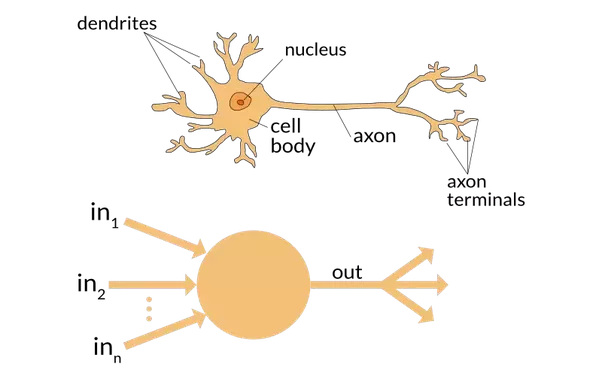
\includegraphics[width=0.6\textwidth]{imgs/walter_pitts.png}
\caption{ Imágen esquemática del modelo de neurona propuesto por \cite{pitts}. Fuente: \cite{fastbook}. }
\label{fig:pitts}
\end{figure}

En 1958 el psicólogo Frank Rosenblatt desarrolla la neurona artificial (Mark I Perceptrón) con habilidad para aprender en \textit{``The Design of an Intelligent Automaton''} \cite{rosenblatt}. El mismo poseía la siguiente formulación (ver figura \ref{fig:perceptron}) \cite{perceptron}:

\begin{equation*}
    o(x_1, ..., x_n) = \left\lbrace\begin{array}{l} ~~1~si~w_0 + w_1 x_1 + w_2 x_2 + ... + w_n x_n > 0 \\ -1~en~caso~contrario \end{array}\right.
\end{equation*}

Los parámetros $w_i$ se inicializarían de manera aleatoria y actualizarían iterativamente comparando la salida $o$ del perceptrón con la salida esperadas $y$, siguiendo la siguiente fórmula: 
\begin{equation*}
    w_i \leftarrow w_i + \Delta w_i
\end{equation*}
\begin{equation*}
    \Delta w_i = \eta (y - o) x_i
\end{equation*}
Donde $x_i$ es el atributo respectivo al peso que se está actualizando y $\eta$ una constante que denominada \textit{learning rate}. En \cite{allen-newell} se ha demostrado que de ser $\eta$ suficientemente pequeña, en un problema binario linealmente separable el algoritmo converge a la solución óptima. El procedimiento es análogo al método de descenso por gradiente que se verá en las próximas secciones y en el cuál se basa la optimización de las actuales redes neuronales.

\begin{figure}[h!]
\centering
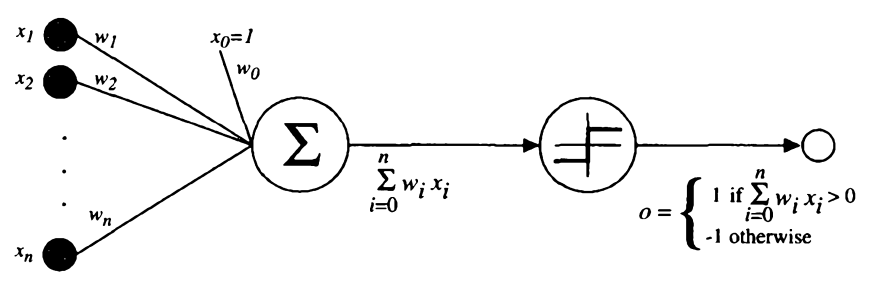
\includegraphics[width=0.6\textwidth]{imgs/perceptron.png}
\caption{ Representación gráfica de un perceptrón. Fuente \cite{perceptron}.  }
\label{fig:perceptron}
\end{figure}

El preceptrón de Rosenbalt cayó en el olvido luego de que una publicación del profesor de MIT (colega de Rosenbaltt) Marvin Minsky demostrara que no podía representar simples funciones como XOR. Este perceptrón puede verse como un hiperplano partiendo el espacio de atributos de manera que produce una salida igual a 1 para instancias que se encuentran a un lado del hiperplano, y -1 al otro. Por eso la efectividad está limitada a conjuntos de datos linealmente separables. \\


Otro antecedente histórico de imitar la estructura de comportamiento del cerebro se haya en \textit{``Parallel Distributed Processing (PDP)''} \cite{PDP} donde se describe que de existir un sistema tal, poseería las siguientes características (todas características que poseen las redes neuronales actualmente):
\begin{enumerate}
    \item Un conjunto de unidades de procesamiento.
    \item Un estado de activación de las mismas.
    \item Una función de salida de cada unidad de procesamiento.
    \item Un patrón de conectividad de dichas unidades.
    \item Una regla de propagación de las activaciones a través de la red de conexiones (forma de transformar las salidas de una unidad en entradas de la otra).
    \item  Una regla de activación para combinar las entradas de las unidades, el estado actual y producir las salidas de la unidad.
    \item Una regla de aprendizaje donde se modifican los patrones de conectividad por medio de la experiencia.
    \item Un entorno en donde el sistema opera.
\end{enumerate}

Durante la década del 80' las redes neuronales vuelven a cobrar cierta tracción en el mundo científico a raíz de que se demostrara que agregar una segunda capa de neuronas evitaría el problema identificado por Minsky \cite{universal-width}. Véase figura \ref{fig:one-layer} \\

\begin{figure}[h!]
\centering
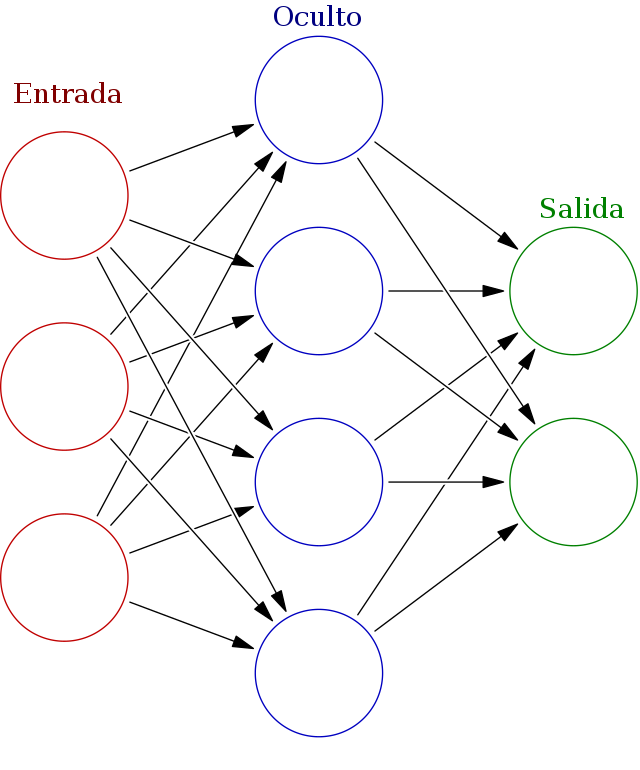
\includegraphics[width=0.4\textwidth]{imgs/one_layer.png}
\caption{ Esquema de red de una capa oculta. Las entradas se combinan linealmente y se le aplica una función no lineal para obtener las activaciones ocultas (valores intermedios) que luego se vuelven a combinar linealmene y aplicar una función no lineal para obtener las salidas o predicciones.  
Créditos de la imágen: \url{es.wikipedia.org/wiki/Red_neuronal_artificial} }
\label{fig:one-layer}
\end{figure}

En 1986 se publicaron los reconocidos trabajos sobre el método de \textit{backpropagation} donde se establece el algoritmo de optimización que hasta el día de hoy es utilizado (con algunas variaciones y ajustes) para entrenar las redes neuronales de muchas capas \cite{backpropagation1} y \cite{backpropagation2}. No obstante actualmente se sabe que esta técnica fue varias veces re-descubierta e incluso existe un antecedente que data de 1960 \cite{backpropagation3}.\\

Si bien teóricamente cualquier función continua puede ser aproximada por redes con una capa oculta con un número suficiente de neuronas se falló en entender la naturaleza fundamentalmente empírica del aprendizaje automatizado y poco se exploró aproximadamente hasta 20 años después sobre el potencial de agregar más capas. 
A fines de los 90' se publica el famoso trabajo \cite{lenet} que mejora sustancialmente la performance utilizando un modelo relativamente sencillo (LeNet-1) y sin extracción manual de caraceterísticas. Fue este el nacimiento de las redes convolucionales que revolucionaron el mundo de la visión computarizada.

\subsection{Formulación actual} \label{subsection:nn-formulacion}

La formulación actual de las Redes Neuronales Artificiales no dista demasiado del modelo simplista de red de una capa oculta, descripto en la subsección anteior. Ver figura \ref{fig:one-layer}. 

Supongamos que la función a aproximar es: 
\begin{equation*}
\hat{f} : \mathbb{R}^{n_{in}} \rightarrow \mathbb{R}^{n_{out}}
\end{equation*}
O sea que tenemos $n_{in}$ atributos de entrada y $n_{out}$ de salida.


Una Red Neuronal Artificial consiste escencialmente en transformar el vector de entradas $\{x_i\}_{i=1}^{n_{in}}$ aplicando sucesivamente funciones no lineales $f^j$ denominadas \textbf{capas}. Estas funciones tienen la forma:
\begin{equation*}
    f^j : \mathbb{R}^{w_{j-1}} \rightarrow \mathbb{R}^{w_j}
\end{equation*}

O sea, son simples transformaciones de vectores en vectores. Notaremos $\bar{h}^j = \{h_i^j\}_{i=1}^{w_j}$ el resultado de la $j$-ésima capa. Los resultados de cada capa son denominados \textbf{activaciones} \cite{libro-nielsen}. 

Definiendo $\bar{h}^0 = x$ que constituye la entrada de nuestra red y a menudo se la llama \textbf{capa de entrada}. 

A la dimensión de la capa $\bar{h}^j$, notada $w_j$ se la conoce como \textbf{anchura de la capa}.


Cada una de dichas funciones (capas, de ahora en más) consiste en una transformación afín de la salida de la capa anterior (o el vector de entrada para el caso de la primer capa), seguida de una función no lineal $\phi^j$ (denominada \textbf{función de activación}). 


Los modelos donde la información fluye desde la entrada hasta la salida sin retroalimentaciones se denominan \textit{\textbf{feed forward}} (ver figura \ref{fig:feedforward}). 

Suponiendo que tenemos $m$ capas, el vector de las $\{h_i^m\}_{i=1}^{n_{out}}$ constituyen la salida de nuestra red. El número $m$ de capas se denomina \textbf{profundidad}.

Podemos formular una red neuronal \textit{feed forward} más formalmente -y de forma concisa- como:

\begin{equation*}
    \bar{h^0} = \bar{x}
\end{equation*}
\begin{equation*}
    \bar{h}^{j+1} = f^{j+1}(\bar{h}^j)
\end{equation*}
\begin{equation*}
    out_i = h_i^m ~ 0 \leq i < n_{out}
\end{equation*}
Donde:
\begin{equation*}
    f^j(\bar{h}^{j-1}) = \phi^j( {W^j}^\top \bar{h}^{j-1} + b^j)
\end{equation*}

\begin{figure}[h!]
\centering
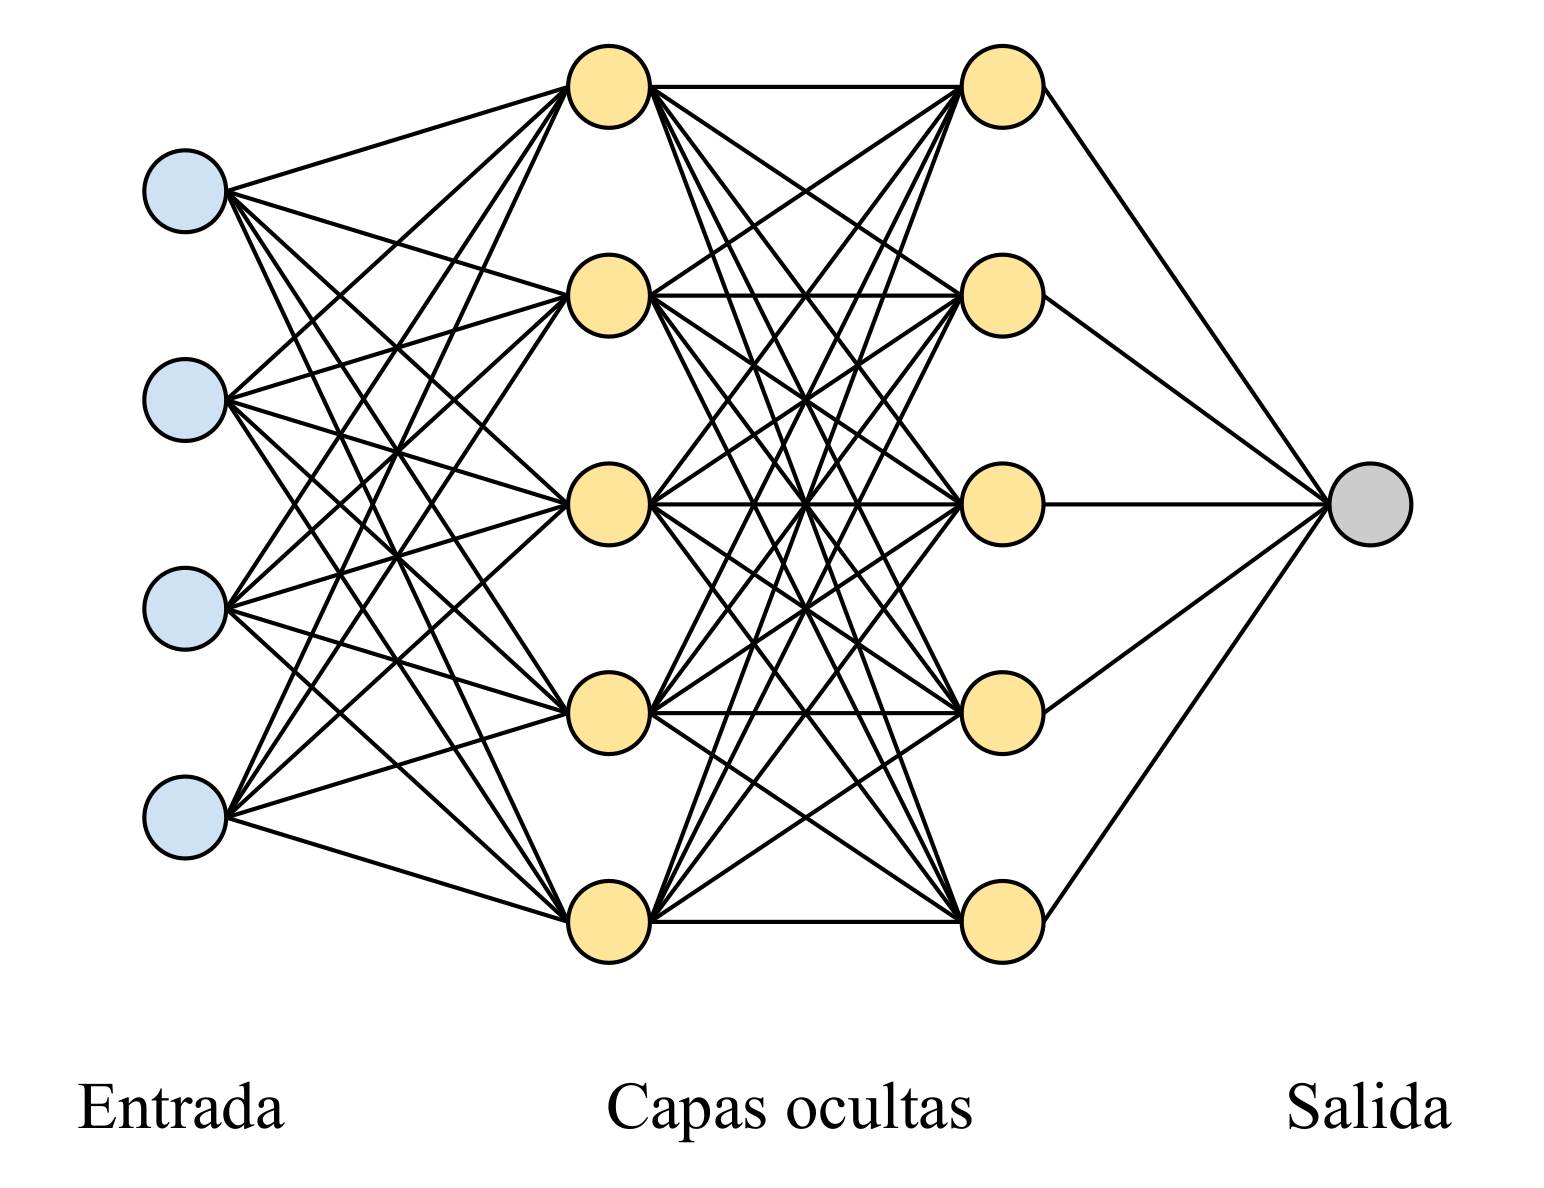
\includegraphics[width=0.4\textwidth]{imgs/feedforward.png}
\caption{ Esquema de un modelo de red neuronal \textit{feed forward}. Análogamente a los modelos de una única capa oculta, las entradas se combinan linealmente y se le aplica una función no lineal para obtener activaciones ocultas. Existe un vector de activaciones ocultas por cada capa de valores intermedios (capa oculta) que resulta de combinar linealmente y aplicar una función no lineal sobre la capa anterior. Finalmente la última capa constituye la salida del modelo. Imágen extraída de \cite{tesina-marcos} }
\label{fig:feedforward}
\end{figure}

Los valores de las matrices $W^j \in \mathbb{R}^{w_{j-1} \times w_j}$, $b^j \in \mathbb{R}^{w_j}$ son los parámetros a entrenar y se denominan respectivamente \textbf{pesos} y \textit{\textbf{biases}} en la jerga del aprendizaje profundo. Son responsables del cambio de dimensión de una capa a otra de activaciones aplicando una transformación afín. La función de activación $\phi^j$ generalmente es una simple función $\mathbb{R} \rightarrow \mathbb{R}$ que es aplicada de forma independiente componente a componente. 

Fijado el número $m$ de capas, sus respectivas anchuras $w_j$ y funciones de activación $\phi^j$ queda definida ``el esquema'' de la red: la cantidad de parámetros y su relación con las entradas queda fija. Las salidas solo dependerán de la elección de los parámetros. Ésto es lo que se conoce como \textbf{arquitectura} del modelo o red.\\

\sout{\textbf{Nota:} El Aprendizaje Profundo posee una jerga entrevesada para conceptos realmente simples. A menudo ésto ocurre a raíz de llamar de manera \textit{vistosa} ciertos conceptos que ya existían para que suenen más innovadores a lo largo de las publicaciones que los han popularizado. Hay que evitar que esta jerga científica nos haga perder de vista la simpleza de los conceptos subyacentes del Aprendizaje Profundo: \textbf{función de activación} no es más que una función no lineal, \textbf{activaciones} son resultados parciales. En las secciones subsiguientes se seguirán introduciendo conceptos con nombres estrambóticos que tienen significados muy simples como las \textbf{unidades rectificadoras} que son simplemente la función $max(0,x)$. ¡Los principios matemáticos detrás de las Redes Neuronales Artificiales son realmente simples! \\}

\textbf{Observación:} Con los conceptos definidos tenemos un panorma de Red Neuronal Artificial que satisface casi todos los puntos que en \textit{``Parallel Distributed Processing (PDP)''} \cite{PDP} se planteaba como necesario para \textit{``imitar al cerebro humano''}. Tan sólo nos falta tener una forma de evaluar la experiencia y una regla de aprendizaje, que es lo que veremos en las secciones siguientes.

\subsection{Descenso por gradiente} \label{subsection:descenso-gradiente}

En esta sección describiremos la \textbf{regla de aprendizaje} utilizada para \textit{ajustar} el modelo. Definida la arquitectura de una red neuronal, resta elegir valores óptimos de los parámetros $W^j$, $b^j$. Por simplicidad notaremos para esta sección al conjunto de todos los parámetros (\textit{pesos} y \textit{biases}) con $W$. Primero que nada necesitamos definir precisamente qué queremos optimizar. Supongamos que poseemos una función $J$ para medir el error de nuestro modelo al aproximar la función objetivo dada una determinada asignación de pesos: 
\begin{equation*}
    J :  \mathbb{R}^{|W|} \rightarrow \mathbb{R}_0^+
\end{equation*}

Por ahora podemos pensar que $J$ calculará las predicciones (salidas de la red) para cada ejemplo del conjunto de datos y lo comparará \textit{de alguna forma} con las salidas esperadas. \\

\textbf{Nota}: notar que $J$ recibe como entrada los \textit{parámetros} del modelo. El conjunto de datos de evaluación (que será provisto como entrada al modelo) se considera fijo para el análisis de $J$. El conjunto de datos no es una entrada de la función $J$.\\

Las funciones que se utilizan para medir el error, comparando las entradas y las salidas son llamadas \textbf{funciones de costo}. En la sección siguiente se habla de qué funciones de costo se usan para cada problema y qué diferencia tiene con el concepto ya definido de \textit{métricas}. 

El método de actualización se basa en el gradiente\footnote{Recordar que el concepto de \textit{gradiente} para una función $\mathbb{R}^n \rightarrow \mathbb{R}$ es un vector donde cada componente es la derivada de la -única- salida respecto de cada componente de la entrada. \cite{apostol} \cite{math-ml} } de los pesos en función del costo:

\begin{equation*}
    \nabla J(W) = \left ( \frac{\delta J}{\delta W_0}, \frac{\delta J}{\delta W_1} , ... , \frac{\delta J}{\delta W_m}  \right )
\end{equation*}

Gráficamente puede interpretarse al gradiente como la dirección (en el espacio de pesos) donde ocurre el mayor incremento de $J$ de manera local (dentro de un entorno infinitamente pequeño). De manera opuesta $- \nabla J(W)$ determina la dirección de mayor decremento local.

El algoritmo de descenso por gradiente usa esto y actualiza los pesos ``moviéndose'' en la dirección opuesta al gradiente (ver figura \ref{fig:gradiente}):

\begin{equation*}
    W_i \leftarrow W_i - \eta \nabla J_i(W)
\end{equation*}

$\eta$ es una constante positiva llamada \textit{\textbf{learning rate}} que determina cuánto se modifica $W$ en la dirección y magnitud del gradiente del costo. Notar que ésta fórmula es similar a la de actualización del original Perceptrón \cite{perceptron}. \

\begin{figure}[h!]
\centering
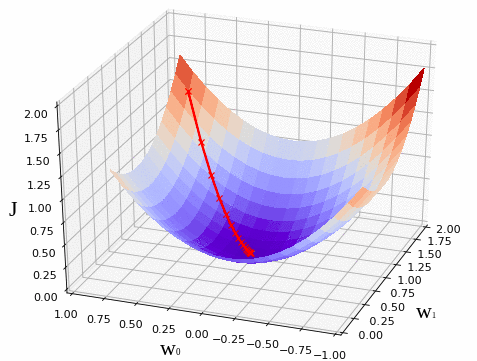
\includegraphics[width=0.6\textwidth]{imgs/descensogradiente.png}
\caption{ Ejemplo de descenso por gradiente en un espacio de dos parámetros para una función de costo convexa. En la práctica los espacios de pesos son de altísima dimensionalidad y las funciones suelen no ser suaves y poseer mínimos locales y puntos de ensilladura. Imágen extraída de \cite{tesina-marcos}  }
\label{fig:gradiente}
\end{figure}

El algoritmo converge cuando se alcanza un punto crítico (gradiente cero). Notar que en casos donde la función no es convexa es posible que el algoritmo converja a \textbf{mínimos locales} (que no sean el mínimo global) o \textbf{puntos de ensilladura} (ver figura \ref{fig:localmin}).

\begin{figure}[h!]
\centering
\begin{subfigure}{0.45\textwidth}
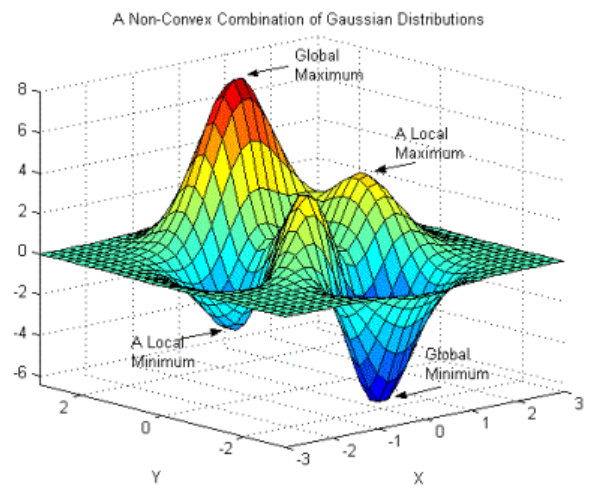
\includegraphics[width=0.4\textwidth]{imgs/localmin.png}
\end{subfigure}
\begin{subfigure}{0.45\textwidth}
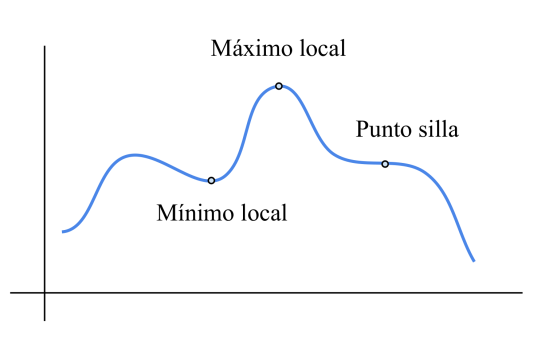
\includegraphics[width=0.4\textwidth]{imgs/critico.png}
\end{subfigure}

\caption{ En la figura izquierda podemos ver un ejemplo de función de dos parámetros no convexa. Se señalaron los mínimos locales. En la figura derecha se muestran los dos tipos de puntos críticos: mínimos y máximos locales, y puntos de ensilladura. El máximo global es un caso particular de éstos. Imágen extraída de \cite{tesina-marcos} y \cite{tesina-zanetti}. }
\label{fig:localmin}
\end{figure}

En la práctica las funciones de costo poseen formas irregulares como muestra el trabajo \cite{visualizing-landscapes}, con varios mínimos locales (ver figura \ref{fig:loss_surface}). Pero se ha corroborado que no encontrar mínimos globales no constituye un problema siempre que se encuentren mínimos locales con bajo costo \cite{deeper-better}. Además \cite{no-chair} muestra que para muchas funciones no convexas de alta dimensionalidad, los mínimos locales son infrecuentes respecto a los puntos ensilladura.

\begin{figure}[h!]
\centering 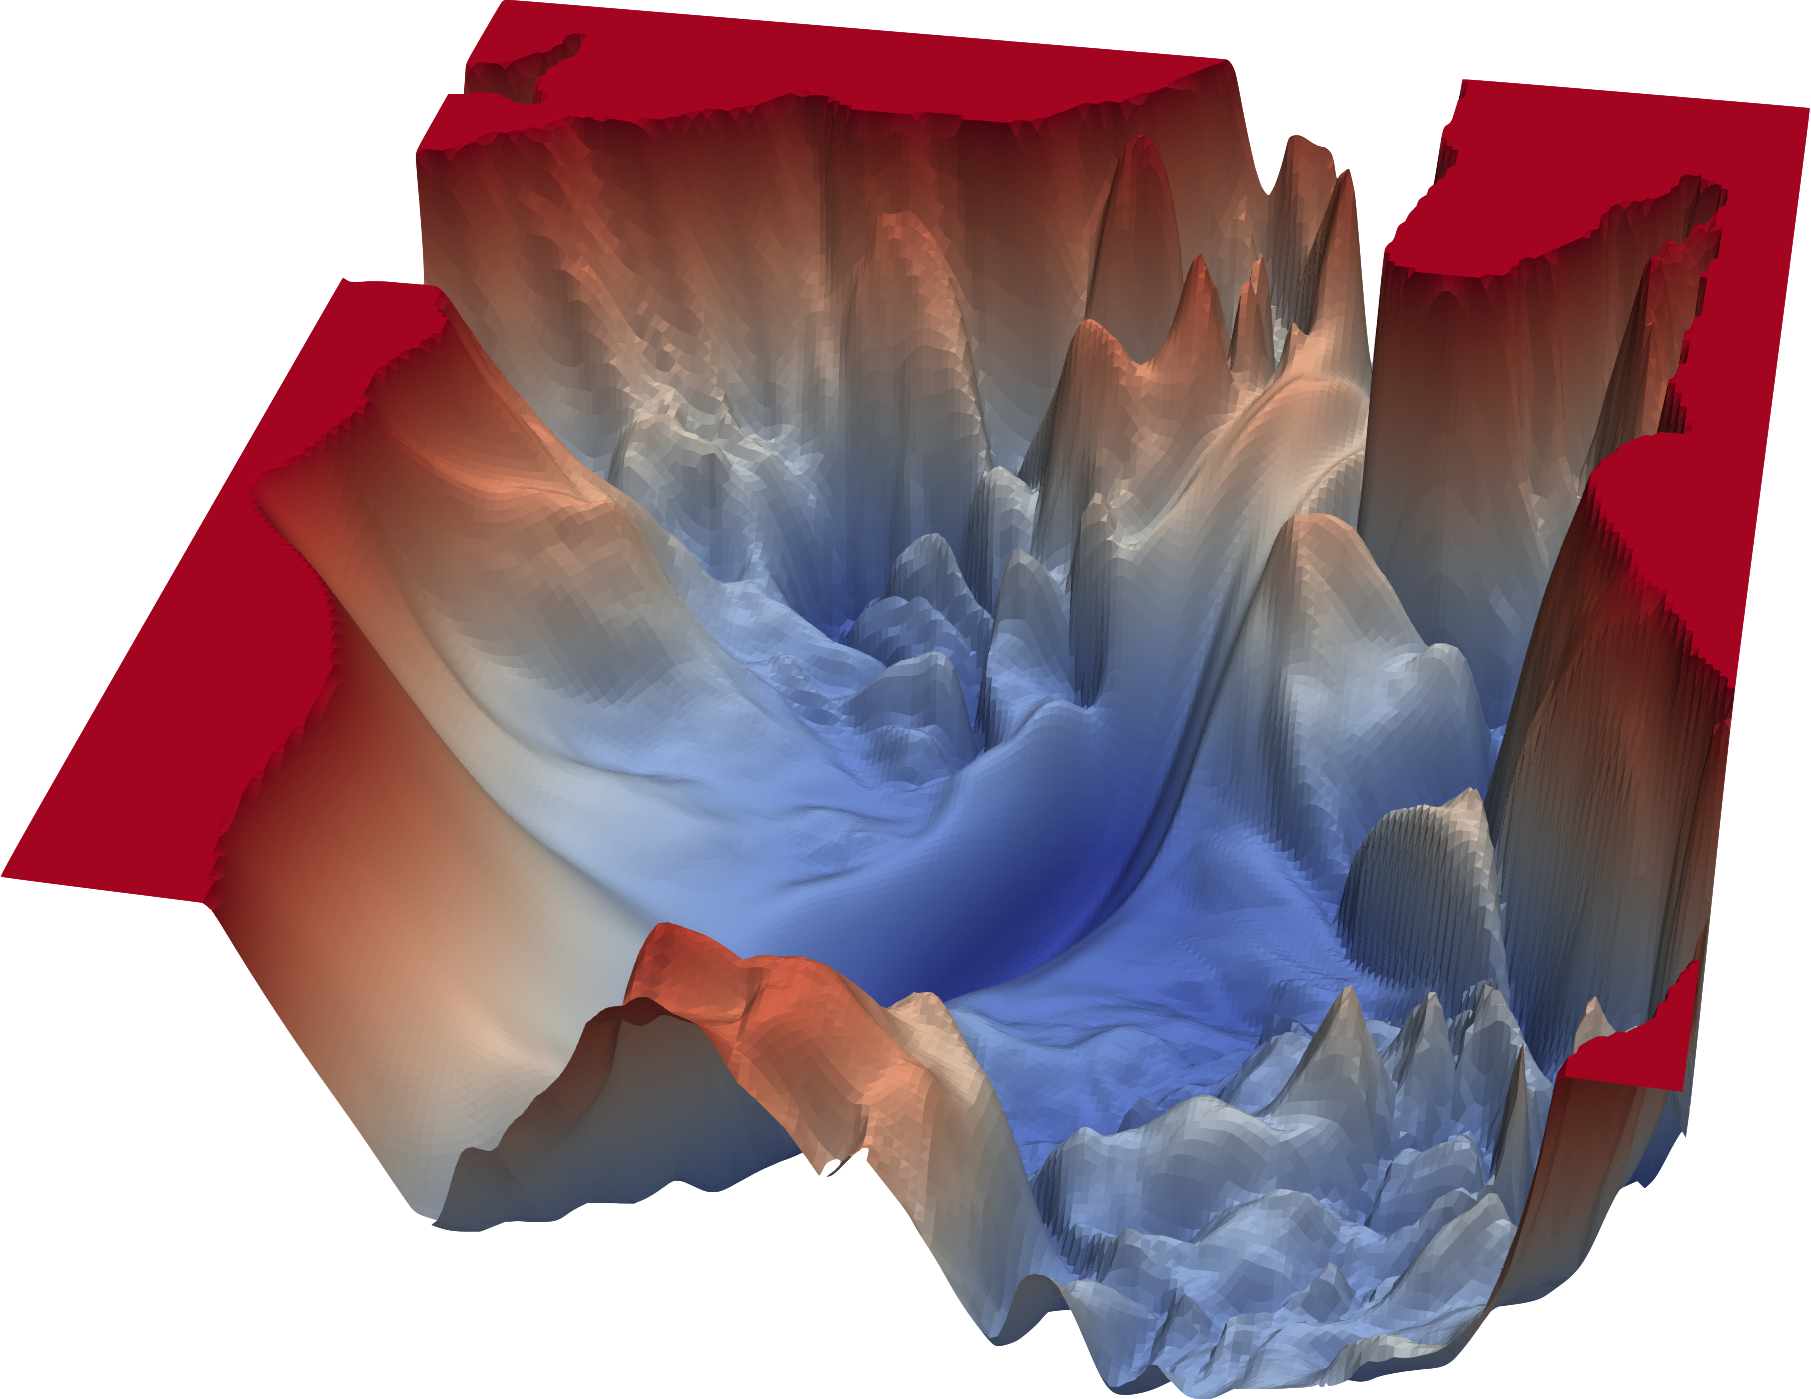
\includegraphics[width=0.4\textwidth]{imgs/loss_surface.png}

\caption{ Visualización en dos dimensiones de la función de costo sobre un conjunto de datos reales. Fuente: \cite{visualizing-landscapes}. }
\label{fig:loss_surface}
\end{figure}

\subsubsection{Sobre funciones de costo ``\textit{realistas}''} \label{subsubsection:sharped-mins}

Las funciones de costo dependen tanto de la arquitectura como del conjunto de datos. Esta característica conceptual tiene una implicancia metodológica en el estudio de las funciones de costo, ya que si bien la arquitectura la controlamos y podemos variar, esto no posible con el conjunto de datos. Las entradas del modelo no poseen una distribución arbitraria sino que está restringido al dominio particular de estudio. 

Si estamos entrenando con el conjunto de fotos de \textit{\textbf{ImageNet}} \cite{imagenet}, las imágenes esperadas en una aplicación final serán fotografías. No esperaremos, por ejemplo, una imágen de un espectrograma de sonido u obras de arte. 

Este concepto es clave ya que a veces se tratan de hacer análisis teóricos sobre funciones de costo arbitrarias cuando las conclusiones clave se han derivado más bien de análisis empíricos de funciones de costo \textit{``realistas''}, o sea, considerando solamente conjuntos de datos reales.

Otra consecuencia es que la función de costo durante la evaluación del modelo no es la función de costo sobre la totalidad del espacio de entrada que idealmente querríamos minimizar. Es importante contar con un conjunto de validación correctamente diseñado que nos garantice que la evaluación sea extrapolable y el modelo generalice bien. Lo mismo ocurre entre las funciones de costo respectivas al conjunto de entrenamiento y evaluación.

La limitación señalada en el párrafo anterior es intrínseca a la finitud de nuestros datos. Es por ello que los resultados han demostrado que más importante que encontrar mínimos globales, es el hecho de encontrar \textbf{mínimos suaves}, de modo que pequeñas diferencias entre las funciones de costo (al tratarse de conjuntos de datos distintos y por ende funciones distintas) supongan pocas variaciones entre los respectivos costos. Ver figura \ref{fig:generalization_loss}.

\begin{figure}[h!]
\centering 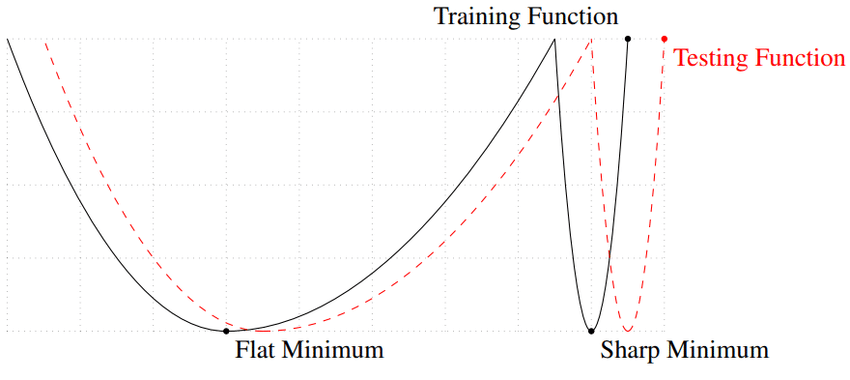
\includegraphics[width=0.5\textwidth]{imgs/generalization_loss.png}
\caption{ Los mínimos suaves supondrán, probablemente, cambios menores en el resultado del costo producto de las variaciones entre funciones de costo al variar los datos, y por ende presentan un \textbf{mayor poder de generalización} que los mínimos afilados. Fuente: \cite{fastbook} }
\label{fig:generalization_loss}
\end{figure}

\subsubsection{Descenso por gradiente estocástico}

Computar el gradiente del error sobre todo el conjunto de entrenamiento es costoso computacionalmente. En la actualidad los conjuntos de datos pueden ser muy grandes: ¡ya el conjunto de datos de imágenes \textit{ImageNet} (\cite{imagenet}) contiene 14 millones de imágenes de resolución considerable! (generalmente se trabaja con  recortes de 224x224 píxeles). Si se gasta demasiado tiempo para \textit{cada actualización} de los pesos el método sería demasiado lento.

Una solución consiste en estimar el gradiente de la función de costo $J$ teniendo en cuenta sólo un subconjunto de los datos de entrada (usualmente denominado \textbf{\textit{mini-batch}} $B$). Como ya dijimos, la función de costo depende de los datos. Podemos pensar, entonces, que estamos calculando el gradiente de la función de costo definida con ese subconjunto de datos $J_B$:

\begin{equation*}
    B \subset D_t
\end{equation*}
\begin{equation*}
    w \leftarrow w - \eta \nabla J_B(w)
\end{equation*}


Se particiona el conjunto de entrenamiento $D_t$ en \textit{mini-batches} y para cada uno se ejecuta un paso denominado \textbf{iteración de entrenamiento}: se evalúa el modelo, se calcula el gradiente del costo y se actualizan los pesos. 
Las iteraciones de todas las particiones constituyen lo que se denomina \textbf{época de entrenamiento}. 
La cantidad de épocas es la cantidad de veces que el modelo ajusta el conjunto de datos de entrenamiento, por lo que al aumentarlo hará más probable que el modelo comience a sobreajustar.

La elección del \textbf{tamaño del \textit{mini-batch}} supone una relación costo beneficio ya que a medida que lo incrementemos:
\begin{itemize}
    \item Cada iteración de entrenamiento consumirá más tiempo y memoria.
    \item El gradiente calculado $\nabla J_B(w)$ será más estable y representará una mejor estimación del gradiente verdadero $\nabla J(w)$ (sobre todo el conjunto de datos).
\end{itemize}

Como el subconjunto de datos que se le suministra al modelo en cada iteración de descenso por gradiente es aleatorio, el método se denomina \textbf{descenso por gradiente estocástico}. La estocasticidad introducida hace que $J_B$ sea distinto entre iteración e iteración y entre épocas sucesivas (ya que cambia $B$). Éstas variaciones suelen ser útiles para evitar mínimos filosos que no generalizan bien.

El hecho de entrenar en \textit{\textbf{mini-batch}} en vez de utilizar un único ejemplo no solo genera gradientes más estables (buenos estimadores del gradiente real) sino que se presta a paralelizar en \textbf{GPU} los cómputos: lo que ha permitido un enorme salto en el desarrollo del Aprendizaje Profundo.

\subsubsection{Importancia de la elección adecuada del \textit{learning rate}} \label{subsubsection:learning-rate}

La elección del \textit{learning rate} ha sido por tiempo uno de los hiperparámetros más importantes a la hora de entrenar redes neuronales. Como podemos ver en la figura \ref{fig:diff-lr}, de ser demasiado pequeño puede generar convergencia muy lenta y de ser demasiado grande también, e incluso, el proceso puede diverger.

\begin{figure}[h!]
\begin{subfigure}{0.33\textwidth}
\centering 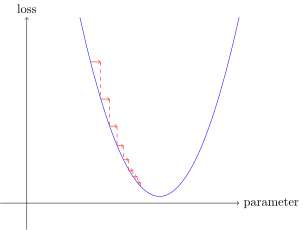
\includegraphics[width=0.3\textwidth]{imgs/lr_small.png}
\end{subfigure}
\begin{subfigure}{0.33\textwidth}
\centering 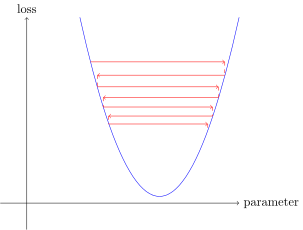
\includegraphics[width=0.3\textwidth]{imgs/lr_big1.png}
\end{subfigure}
\begin{subfigure}{0.33\textwidth}
\centering 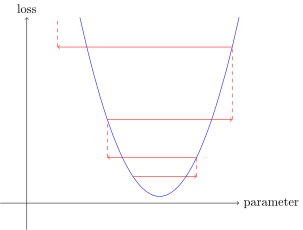
\includegraphics[width=0.3\textwidth]{imgs/lr_big2.png}
\end{subfigure}
\caption{ La elección del \textit{learning rate} es importante para la convergencia del método de manera eficiente. Fuente: \cite{fastbook} }
\label{fig:diff-lr}
\end{figure}


Más adelante se mostrarán optimizaciones más avanzadas que se basan en descenso por gradiente pero ajustan el \textit{learning rate} conforme avanza el entrenamiento. También existen heurísticas que permiten tomar decisiones razonables para la elección del mismo.

Es importante volver a resaltar que como la estabilidad de los gradientes calculados dependen del \textbf{tamaño de \textit{mini-batch}}, de éste dependerá el valor óptimo de \textit{learning rate}.

\subsection{Función de costo}

En el capítulo anterior asumimos que poseíamos una función que calculase el error para una asignación de parámetros determinada: 
\begin{equation*}
    J :  \mathbb{R}^{|W|} \rightarrow \mathbb{R}_0^+
\end{equation*}
A dicha función la nombramos \textbf{función de costo}. Luego introducimos un algoritmo para optimizarla, que se basa en el cálculo de $ \nabla J $. 

¿Por qué no usar las ya introducidas \textbf{métricas} como funciones de costo? 
Una de las razones es que sus gradientes no poseen buenas propiedades por lo que no se ajusta bien a nuestro algoritmo de aprendizaje.

Las métricas tales como la \textit{tasa de aciertos} son funciones escalonadas: un pequeño cambio en los pesos generará un cambio en las probabilidades de la predicción pero muy probablemente no cambiará la clase predecida, y por ende en la tasa de aciertos no se modificará. O sea el gradiente será nulo.

En cambio se utilizan como funciones de costo:
\begin{itemize}
    \item En problemas de \textbf{regresión} el ya definido \textbf{Error Cuadrático Medio} (\textbf{MSE}).
    
    Además de ser una función diferenciable, presenta buenas propiedades de concavidad.

    \item En problemas de clasificación binaria \textbf{\textit{Binary Cross Entropy}} \footnote{Centraremos nuestro análisis en \textit{BCE} ya que, como se dijo, el problema a tratar en este trabajo es de clasificación binaria. No obstante el concepto de \textit{BCE} se extiende fácilmente (y también sus propiedades) a la función de costo \textit{Cross Entropy Loss} para problemas de clasificación de cantidad arbitraria de clases.} (\textbf{BCE}):
    
    \begin{equation*}
        BCE(y, p) = \sum_{x_i \in D_v} y_i~log(p_i) + (1-y_i)~log(1-p_i)
    \end{equation*}
    
    \textbf{Observación:} como $y_i \in \{0,1\}$ (clasificación binaria), las expresiones $y_i$ y $1-y_i$ simplemente cumplen el rol de ``elegir'' que término sumar: $log(p_i)$ o $log(1-p_i)$ respectivamente.
    
    Intuitivamente podemos pensar que si el $log$ no estuviera es una \textit{``tasa de aciertos''} continua que mide que distancia hay entre la probabilidad predecida y la predicción correcta. El efecto del $log$ hace que la función pondere adecuadamente la diferencia entre clasificar, por ejemplo, con un error de $0.001$ y $0.01$ (en términos absolutos no es mucho pero en términos de error es $10 \times$ mejor).
    
    Es un caso particular de la función de entropía cruzada (en inglés \textit{Cross Entropy Loss}), utilizada en probabilidad para calcular diferencia entre distribuciones, con bases en la teoría de la información \cite{math-ml}.
    
\end{itemize}

Otro sustento matemático a la elección de dichas funciones de error es que sus fórmulas se derivan de los estimadores de máxima probabilidad (\textit{Max Likelihood Estimators}). 

\subsubsection{Linearidad de gradientes respecto a última capa de activaciones}

Una propiedad interesante surge de analizar $ \frac{\delta J}{\delta z} $ siendo $z$ la última capa de activaciones.\\

En problmeas de clasificación generalmente tendremos: \footnote{La nombrada \textit{función sigmoide} es una función de activación utilizada frecuentemente en la última capa para problemas de clasificación binaria. Se verá con más detalle en \ref{subsection:activaciones}. }
\begin{equation*}
    J(W) = BCE(y, sigmoid(z))
\end{equation*}
Y los gradientes respecto a la última capa de activaciones serán:
\begin{equation*}
    \frac{\delta J}{\delta z} = sigmoid(z) - y
\end{equation*}

En problemas de regresión simplemente será:
\begin{equation*}
    J(W) = MSE(y, z)
\end{equation*}
Y los gradientes respecto a la última capa de activaciones serán:
\begin{equation*}
    \frac{\delta J}{\delta z} = 2 (z - y)
\end{equation*}

En ambos casos los gradientes respecto a la última capa de activaciones serán proporcionales a la diferencia entre la predicción y el objetivo. 
Ésto hace que dicho gradiente que se ``propagará'' (como ya veremos en el capítulo de \textit{backpropagation}) hacia las capas anteriores no poseerá saltos bruscos: se \textit{suavizará} al aproximarse al objetivo tanto como se acerque al mismo. Sería problemático, si por el contrario aumentara exponencialmente al alejarse del objetivo, ya que, intuitivamente hablando, podría dar pasos tan grandes que saltase muy por ensima del mínimo y diverger (ver figura \ref{fig:diff-lr}). Notar que también sería un problema si no disminuyese conforme se acercase al mismo, ya que en un entorno próximo al mismo son necesarios pasos cada vez más pequeños.

\subsection{Funciones de activación} \label{subsection:activaciones}

Notar la importancia de aplicar funciones no lineales: de no hacerlo la combinación sucesiva de transformaciones afines no sería otra cosa que una transformación afín, y por lo tanto sería inútil la aplicación de sucesivas capas: el modelo sería en su conjunto una simple regresión lineal.

Diferentes funciones de activación utilizadas son:

\begin{figure}[h!]
\centering
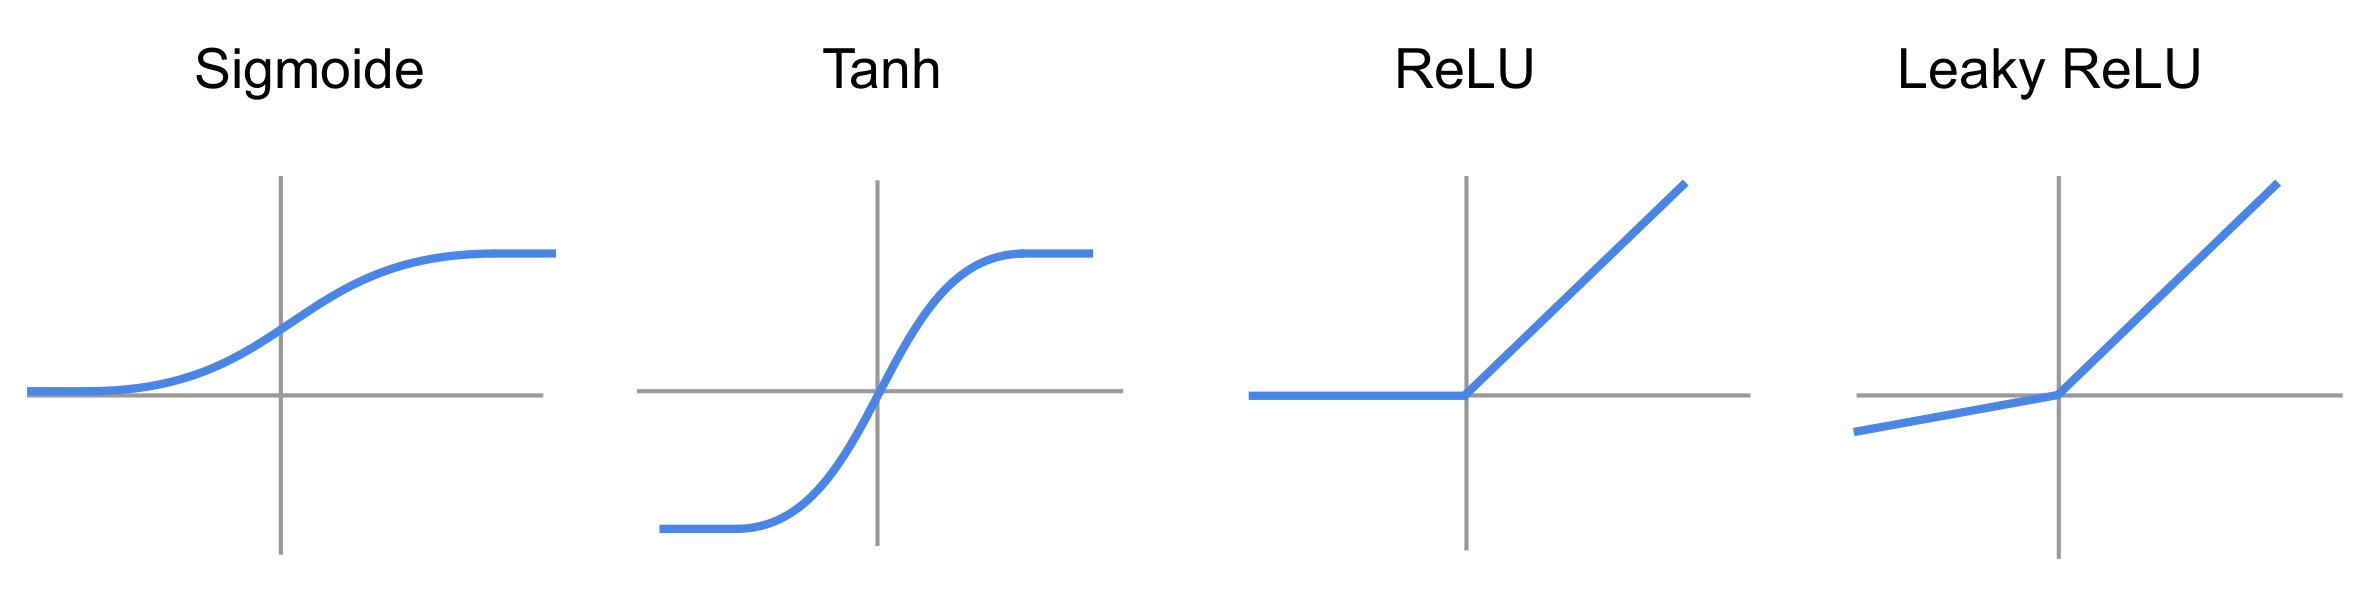
\includegraphics[width=0.8\textwidth]{imgs/activaciones.png}
\caption{ Diferentes alternativas para la función de activación. }
\label{fig:activaciones}
\end{figure}

\begin{itemize}
    \item \textbf{ Sigmoide }($\sigma$):
    \begin{equation*}
        \sigma(x) = \frac{1}{1+e^{-x}}
    \end{equation*}
    Las salidas de las neuronas sigmoideas no están centradas en el cero. Esto puede causar que el gradiente sea siempre positivo o negativo, causando inestabilidad en la actualización de los pesos.
    
    Suele utilizarse, no obstante, sobre la última capa de activaciones (como última función de activación) para problemas de clasificación binaria. De este modo las predicciones son números en el rango $[0,1]$ (consistentes con el hecho de reflejar probabilidades de pertenecer a la clase positiva o negativa). Además, como ya se explicó, posee buenas propiedades con respecto a \textit{BCE} al ser utilizada como última función de activación.
    
    \item \textbf{ Tangente hiperbólica }:
    \begin{equation*}
        tanh(x) = \frac{e^{x}-e^{-x}}{e^{x}+e^{-x}} = \frac{1}{1+e^{-2x}} - 1 = 2\sigma(2x) - 1
    \end{equation*}
    $Tanh$ es una sigmoide escalada y corrida. Resuelve el problema de centro distinto de cero.
    
    Históricamente estas dos funciones surgieron como primeras alternativas por ser diferenciables en todo su dominio, y en continuidad con el concepto de neurona encendida/apagada que poseía el perceptrón originalmente.
    
    Pero éstas funciones poseen el problema que el gradiente (derivada) es prácticamente nulo para valores de fuera del rango de [-2, 2]. Este problema se conoce como ``saturación del gradiente''.
    Ésto puede hacer muy pequeña la actualización de los pesos hacia capas anteriores (lo que se conoce como \textit{señal de backpropagation}) en los casos donde la activación escape al mencionado rango. Este comportamiento es denominado como problema de desvanecimiento del gradiente (en inglés, \textit{gradient vanishing}) y es sobretodo relevante en las actuales \textit{arquitecturas profundas} (que poseen un gran número de capas). Intuitivamente ``no les importa demasiado'' que los pesos de capas anteriores cambien ya que esto no genera cambios sustanciales en la función de activación. Es por eso que ya no se las utiliza como funciones de activación para capas intermedias. 
    
    \item \textit{\textbf{ Rectified Linear Unit}} (ReLU):
    \begin{equation*}
        ReLU(x) = max(0,x)
    \end{equation*}
    
    Las ReLUs fueron introducidas en \cite{relu-def} y sus variantes adquirieron mayor popularidad, mostrando resultados superadores en el entrenamiento de redes profundas debido a que:
    \begin{itemize}
        \item Resuelven el problema de saturación del gradiente.
        \item  Involucran operaciones simples (función $max(0,x)$ a diferencia de sigmoide o $tanh$ que involucran exponenciales), siendo computacionalmente menos costosas.
        \item En \cite{relu-fast} se muestra que son 6 veces más rápidas que sigmoide o $tanh$ para converger utilizando el método de descenso por gradiente estocástico.
        \item En \cite{relu-biology} muestran que las neuronas con ReLUs representan un mejor modelo de las neuronas biológicas y aprenden mejor que $tanh$ o sigmoide las representaciones dispersas.
        \item Es simple demostrar y ver (como veremos cuando hablemos de teorema de aproximación universal) que cualquier función puede ser aproximada como combinación lineal de ReLUs
    \end{itemize}

    Las ReLUs poseen un problema denominado ``neuronas muertas'': el gradiente es $0$ en el rango $(-\infty, 0)$ lo que anula la propagación a las capas anteriores y esto puede generar que conjuntos de neuronas de diversas capas no se activen. Y además, como tampoco actualizan sus respectivos pesos difícilmanete volverán a activarse.
    
    \textit{Leaky ReLU} introducidas en \cite{leaky-relu1} y \cite{leaky-relu2} pretende solucionar este problema agregando una pequeña pendiente en el rango $(-\infty, 0)$.

    
    \item \textit{\textbf{ Leaky ReLU}}:
    \begin{equation*}
        Leaky~ReLU(x) = \left\lbrace\begin{array}{c} \alpha x~si~x<0 \\  x~si~x \geq 0 \end{array}\right.
    \end{equation*}
    Con:
    \begin{equation*}
        0 < \alpha \ll 1
    \end{equation*}
    En general las ReLUs se siguen usando porque \textit{Leaky ReLU} no ha mostrado una mejoría consistente.
    
    \item \textit{\textbf{ Softmax}}: suele utilizarse en la última capa en problmeas de clasificación para transformar activaciones arbitrarias en probabilidades.
    
    \begin{equation*}
        \sigma : \mathbb{R}^K \rightarrow [0,1]^K
    \end{equation*}
    \begin{equation*}
        \sigma(z)_i = \frac{e_{z_i}}{\sum_{j=1}^K e_{z_j}}
    \end{equation*}
    
    Intuitivamente puede pensarse que:
    \begin{itemize}
        \item ``positiviza'' las activaciones y las mapea al rango $[0,1]$.
        \item  hace que la suma de las probabilidades sea $1$ (notar que sirve para problemas de clasificación donde la respuesta es una única clase, no múltiples clases).
        \item amplifica las diferencias entre las activaciones diferentes (tiende a tratar de escoger una única opción).
    \end{itemize}
    
    La elección de esta función tiene bases en la teoría de probabilidad. 
    
    El gradiente en la última capa de activaciones es lineal a la diferencia entre las predicciones y las etiquetas cuando se utilzia \textit{softmax} como última función de activación junto a \textit{BCE} como función de costo (al igual de lo que se mostró que pasaba con \textit{sigmoid}). Cómo se explicó, esto es una propiedad deseada.
    
\end{itemize}

\subsection{Teorema Aproximación Universal}

Como se dijo en la subsección \ref{subsection:intro-redes}, el Perceptrón de Rosenblatt de una sóla neurona cayó en olvido luego de que Marvin Mibsky mostrara que funciones simples como XOR no podían ser representadas. En la década del 80' las redes neuronales se popularizaron nuevamente luego que se demostrara que se podía solucionar dicho problema agregando más de una capa.

Los \textit{Teoremas de Aproximación Universal} son una familia de teoremas que demuestran las capacidadades de las redes neuronales de aproximar \textit{casi} cualquier función. 
No entraremos en detelle sobre la formulación matemática exacta de dichos teoremas (el lector interesado puede encontrar una explicación muy amena en el capítulo 4 de \cite{libro-nielsen}). 

Sólo nombraremos que se demuesta que es posible aproximar cualquier función continua en un espacio compacto de $\mathbb{R}^p$ a un grado de precisión arbitrario con:
\begin{itemize}
    \item \textbf{Dos capas + anchura arbitraria}: dado un número suficiente de neuronas intermedias.

    \item \textbf{Anchura limitada + profundida arbitraria}: con redes suficientemente profundas.
\end{itemize}
El primer caso es muy fácil de demostrar utilizando funciones de activación ReLUs. En la figura \ref{fig:universal-aprox} se muestra un esquema intuitivo. La idea subyacente es dividir el espacio compacto en intervalos y aproximar la función utilizando rectas adecuadas en cada intervalo. A su vez esto es fácil de lograr eligiendo e incorporando a la ecuación $ReLUs$ escaladas y corridas convenientemente para que generen dichas rectas lineales, siempre teniendo en consideración las $ReLUs$ ya elegidas.

\begin{figure}[h!]
\centering
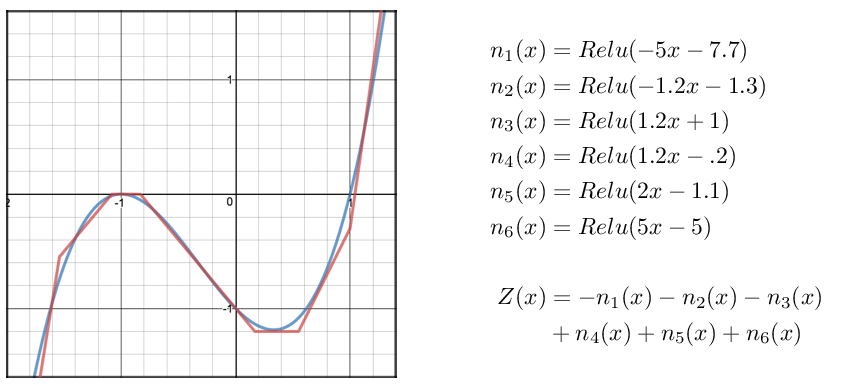
\includegraphics[width=0.8\textwidth]{imgs/universal_aprox.png}
\caption{ La imagen muestra la aproximación de un polinomio de tercer grado con una ``red de dos capas''. Fuente: \url{towardsdatascience.com/can-neural-networks-really-learn-any-function-65e106617fc6}. Autor: Brendan Fortuner }
\label{fig:universal-aprox}
\end{figure}

¡Notar que los teoremas no dan ninguna garantía de que el algoritmo de entrenamiento pueda aprendar esa función! E incluso siempre tendremos el limitante de la finitud de nuestros datos: no existe un procedimiento universal para elegir una función que generalice a puntos fuera del conjunto de entrenamiento \cite{limitation-aprox}.

Grandes errores se han cometido en el desarrollo del aprendizaje profundo por no entender que se trata de una disciplina práctica. En la década del 80' muchos científicos, en base al resultado de los teoremas de aproximación de dos capas, no experimentaron con redes más profundas. En la práctica éstas han mostrado una contundente mayor eficiencia produciendo resultados increíbles \cite{deeper-better}.

Debido al éxito de entrenar redes neuronales con muchas capas es que también nos referimos con un nombre propio al campo que estudia las redes neuronales profundas: \textbf{Aprendizaje Profundo},

\subsection{Algoritmo de \textit{backpropagation}}

En esta sección continuaremos explicando cómo se optimizan los parámetros. Explicaremos como se calculan los gradientes para cada peso siguiendo un algoritmo conocido como \textit{\textbf{backpropagation}}.\\

Ya se mostró que la arquitectura de nuestra red puede verse como composición sucesiva de funciones sobre los datos de entradas. Es natural entonces que para calcular los gradientes nos basaremos en la \textbf{regla de la cadena}. La misma nos dice que si tenemos:

\begin{equation*}
    E_1(w) = f(E_2(w))
\end{equation*}
Luego:
\begin{equation*}
    \frac{\delta E_1}{\delta w}(w) = \frac{\delta f}{\delta E_2}(E_2(w)) . \frac{\delta E_2}{\delta w}(w)
\end{equation*}
Utilizamos la notación de Leibinz extendida para resaltar en qué punto se evalúa cada derivada.\\

\textbf{Nota}: cuando hablamos de gradientes en redes neuronales nos referimos a \textit{valores} y no a las \textit{funciones}. A diferencia de lo que sucede en matemáticas donde es frecuente querer encontrar o calcular la función de gradiente o derivada, en cada iteración del entrenamiento, sólo necesitamos la derivada del error respecto a cada peso \textbf{aplicada en la asignación actual de pesos}.\\
  
En un principio, cuando las arquitecturas eran simples, dichas derivadas se calculaban con una fórmula codificada a mano para cada matriz $W^j$, $b^j$.  Pero si se observa con atención, la regla de la cadena nos da una forma inductiva de calcular los gradientes del error respecto de cada capa, haciendo uso de los gradientes ya calculados de capas posteriores.

Matemáticamente si tenemos las capas $f^1$, $f^2$ ... $f^n$ y las aplicamos sucesivamente según:
\begin{equation*}
    out = f^n ( ... f^2 ( f^1 (x) ) )
\end{equation*}
Y recordamos la notación para las activaciones tal como la definimos en la subsección \ref{subsection:nn-formulacion}:
\begin{equation*}
    \bar{h^0} = \bar{x}
\end{equation*}
\begin{equation*}
    \bar{h}^{j+1} = f^{j+1}(\bar{h}^j)
\end{equation*}

Luego podemos calcular los gradientes $\frac{\delta J}{\delta h^j}$ como:
\begin{equation*}
    \frac{\delta J}{\delta h^j} = \frac{\delta J}{\delta h^{j+1}}(h^{j+1}) . \frac{\delta h^{j+1}}{\delta h^j}(h^j)
\end{equation*}
Esta fórmula nos da una forma constructiva (algorítimica) de calcular los gradientes respecto de cada una de las activaciones, empezando por las capas más profundas (más cercanas al resultado) y conociendo la derivada $\frac{\delta h^{j+1}}{\delta h^j}(h^j)$ de la fórmula que computa una activación a partir de la anterior.  

Una vez que los gradientes respecto a cada capa ${h}^{j}$ han sido calculados, se puede computar de manera simple el gradiente respecto a los parámetros (pesos $W^j$ y \textit{biases} $b^j$) intervinientes en las respectiva capa. \cite{lecun-dl}. Simplemente, conociendo la derivada de $\phi^j$, podemos calcular $\frac{\delta J}{\delta W^j}$ y $\frac{\delta J}{\delta b^j}$ -en función del ya conocido $\frac{\delta J}{\delta h^j}$- valiéndonos de la fórmula de la capa:

\begin{equation*}
    \bar{h}^j = f^j(\bar{h}^{j-1}) = \phi^j( {W^j}^\top \bar{h}^{j-1} + b^j)
\end{equation*}

En éste cálculo la información fluye ``\textit{hacia atrás}'' y es por eso que se denomina \textbf{algoritmo de \textit{backpropagation}} \cite{backpropagation1}. En contraste a éste concepto se llama \textbf{\textit{forward propagation}} al cáclulo de las predicciones, ya que la información en este caso fluye ``\textit{hacia adelante}''.

Notar que en los cálculos intervienen los valores $h_j$, lo que significa que muchas veces será necesario guardar el valor de las activaciones (o al menos cierta información de ellas) para el cálculo posterior de los gradientes. \\

\textbf{Nota}: ¡El algoritmo de backpropagation es un caso de uso de programación dinámica! Estamos usando los resultados de instancias más chicas, o sea de las capas más cercanas al error, para calcular los casos ``más complejos'' de las capas menos profundas. \\

El mismo razonamiento es fácilmente generalizable a cualquier grafo acíclico de computaciones. Ésto es lo que usan los frameworks actuales para calcular los gradientes de manera transparente al usuario: en general no necesitaremos calcular ningún gradiente a mano. Cada una de las funciones definidas, definen un método para calcular los gradientes respecto de sus entradas utilizando como dato los gradientes respecto a esa misma capa. Los frameworks calculan un grafo de ejecucción que lleva el rastro de cómo se fue calculando determinado resultado. De modo que una vez calculado el error (o la función sobre la que queremos calcular los gradientes) es fácil calcular el gradiente de dicha función respecto cada capa (y luego de cada parámetro) haciendo uso de programación dinámica (\textit{backproapagation}) sobre el DAG de ejecucción que calculó el error. Ver esquema en la figura \ref{fig:dag}

\begin{figure}[h!]
\centering
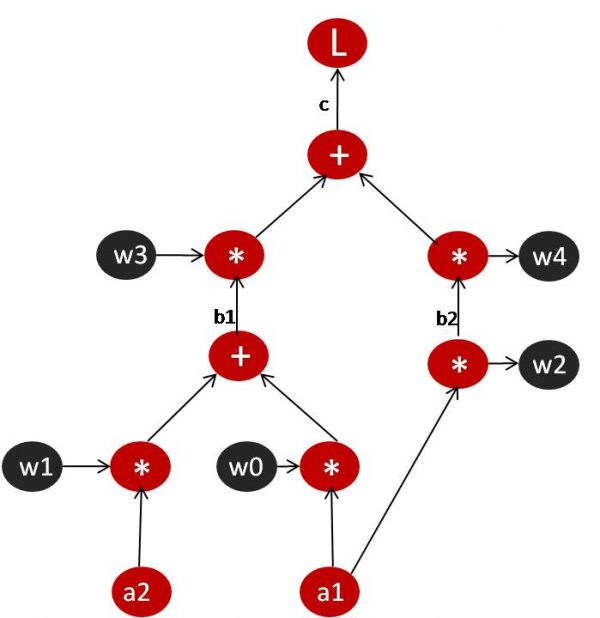
\includegraphics[width=0.4\textwidth]{imgs/autograd.jpg}
\caption{ Ejemplo de grafo de ejecucción construído en base al cálculo de un expresión. Créditos de la imágen: \url{mlearninglab.com/2019/04/14/autograd-una-de-las-claves-de-la-flexibilidad-de-pytorch/} }
\label{fig:dag}
\end{figure}

\subsection{Extensiones al algoritmo de descenso por gradiente}

En esta subsección explicaremos algunas optimizaciones que se hacen al algoritmo de descenso por gradiente estocástico para mejorar su estabilidad y convergencia. Las mismas, conforme avanza el entrenamiento, van adaptando y calculando valores que influyen en la actualización de los pesos. 

Generalmente estas optimizaciones ya vienen integradas en las bibliotecas que permiten crear y entrenar modelos de redes neuronales (como Pytorch y Tensorflow) y han sido utilizadas en el presente trabajo.

Notaremos $t$ al número de iteración y $w_t$ a los pesos al comienzo de la $t$-ésima iteración.

Una lista más extensa y comparaciones de las diferetnes optimizaciones se puede encontrar en \cite{compare-optimizers}.

\subsubsection{Momentum} \label{subsubsection:momentum}

Esta extensión fue propuesta en \cite{momentum}. Consiste en ``recordar'' información de las actualizaciones de pesos de iteraciones anteriores, calculando una media móvil exponencial de las actualizaciones $m_t$, ponderada por un hiperparámetro $\beta$:
\begin{equation*}
    m_t = \beta~m_{t-1} + (1-\beta) (- \eta~\nabla J(w_t))
\end{equation*}
\begin{equation*}
    w_{t+1} = w_t + m_t
\end{equation*}

Intuitivamente puede pensarse que el descenso por gradiente tendrá una \textit{inercia a la dirección que ya poseía}, de ahí que se lo llame \textbf{momentum} (por momento de inercia).

\subsubsection{RMSProp}

\textbf{RMSProp} (por \textit{Root Mean Square Propagation}) fue introducido por \cite{rmsprop}. Propone utilizar un \textit{learning rate} para cada parámetro de modo que los que \textit{``necesitan cambiar más''} posean valores más altos.

Esto lo logra mirando los gradientes, asumiendo que parámetros con gradientes más cercanos a 0 necesitan un \textit{learning rate} más alto para salirse de zonas planas. En cambio, si los gradientes son altos en valor absoluto significa que estamos en zonas empinadas, dónde conviene moderar el \textit{learning rate} para evitar divergencia. El factor que mide cuánto se tiene que reducir el \textit{learning rate} se lo nota $v_t$ (y es diferente para cada peso).

Para que $v_t$ no sea ruidoso (cambie demasiado entre iteraciones) y, en cambio, determinar una tendencia general del valor absoluto de los gradientes, se calcula la siguiente media móvil exponencial:


\begin{equation*}
    v_t = \beta v_{t-1} + (1-\beta) (\nabla J(w_t))^2
\end{equation*}
\begin{equation*}
    w_{t+1} = w_t - \frac{\eta}{\sqrt{v_t + \epsilon}} \nabla J (w_t)
\end{equation*}

Se agrega $\epsilon$ por razones de estabilidad numérica para evitar un denominador nulo.

\subsubsection{Adam} \label{subsubection:adams}

Debe su nombre a \textit{Adaptive Moment Estimation} y es una combinación de Momento y RMSProp propuesta en \cite{adam}. 

\begin{equation*}
    m_t = \beta_1 m_{t-1} + (1-\beta_1) \nabla J(w_t)
\end{equation*}

\begin{equation*}
    v_t = \beta_2 v_{t-1} + (1-\beta_2) \nabla (J(w_t))^2
\end{equation*}

Adam utiliza la media móvil no sesgada en su fórmula final. De modo que corrije el sesgo a $0$ existente en las medias móviles desde el inicio, al ser inicializadas en 0. Este sesgo es especialmente fuerte si $\beta_1$, $\beta_2$ son cercanos a 1 (como los valores que sugiere \cite{adam}). 

$\hat{m}_t$ y $\hat{v}_t$ son los estimadores no sesgados respecto a las medias móviles $m_t$ y $v_t$:

\begin{equation*}
    \hat{m}_t = \frac{m_t}{1-(\beta_1)^{t}}
\end{equation*}


\begin{equation*}
    \hat{v}_t = \frac{v_t}{1-(\beta_2)^{t}}
\end{equation*}

Finalmente la actualización de los pesos se calcula según:

\begin{equation*}
    w_{t+1} = w_t - \frac{\eta}{\sqrt{\hat{v}_t+\epsilon}} \hat{m}_t
\end{equation*}


\subsection{Inicialización de los parámetros}

Como explica el capítulo 17 de \cite{fastbook}, es importante la inicialización correcta de los pesos, sobretodo en redes profundas ya que se calculan muchas multiplicaciones sucesivas de las entradas con ellos. De inicializarlos muy pequeños (en valor absoluto) puede que las activaciones se anulen luego de sucesivas capas. Además, de iniciarlizarlos con valores absolutos demasiado altos (como las ReLU no limitan la saldia de cada capa), puede que incrementen exponencialmente el valor de las activaciones llegando a resultados computacionalmente inmanegables (valores \textit{nan}, de \textit{``not a number''}) causando errores de desbordameinto (\textit{overflow errors})

En \cite{xavier-init} se determina que la escala adecuada para inicializar los pesos es $\frac{1}{\sqrt{n_{in}}}$ siendo $n_{in}$ la cantidad de entradas de la capa. La \textbf{inicialización Xavier} inicializa los pesos en valores aleatorios con distribución gaussiana de media 0 y varianza $\frac{1}{\sqrt{n_{in}}}$.

Este factor depende del tipo de función de activación utilizada y \cite{xavier-init} lo han probado para $tanh$. En \cite{kaiming-init} (mismo trabajo que introduce las redes residuales) determina que la escala en caso de utilizar $ReLU$ es $\sqrt{\frac{2}{n_{in}}}$. Esta es la escala que utiliza el método de \textbf{inicialización Kaiming}.

\subsection{Mejorando la generalización - técnicas de regularización}

Otro desafío que supone el entrenamiento de redes neuronales es el del \textbf{sobreajuste}. Su gran complejidad, consecuencia de la gran cantidad de parámetros posibilita aprender funciones complejas pero también hace que sean más suceptibles a sobreajustar.

A veces se piensa -erróneamente- que la solución adecuada en estos casos es simplificar el modelo (reducir la cantidad de parámetros), la práctica del aprendizaje profundo desvela que es la última de las opciones a la hora de combatir el sobreajuste.

Existen una multitud de técnicas conocidas cómo \textbf{técnicas de regularización}, que permiten modificar el algoritmo de aprendizaje para producir modelos que generalicen mejor, sin achicar la cantidad de parámetros.

\begin{figure}[h!]
\centering
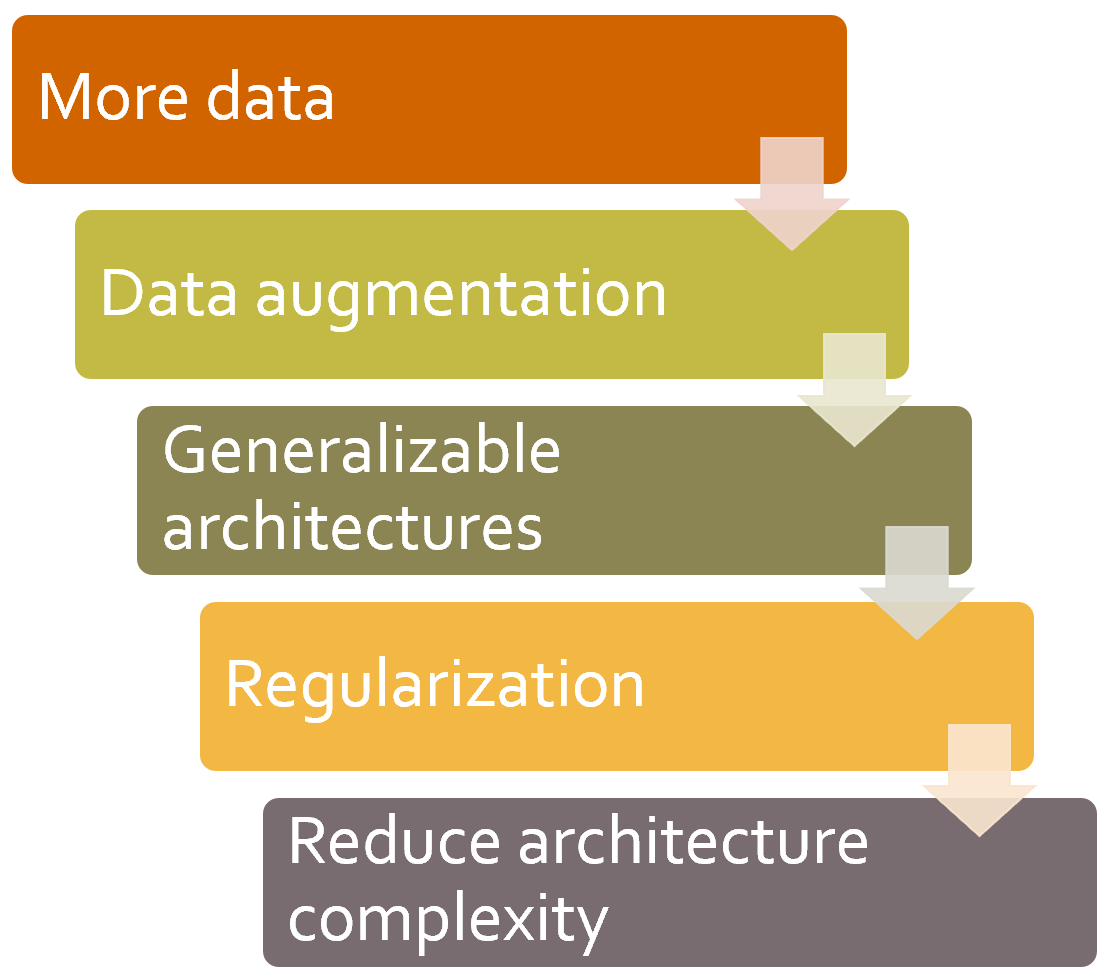
\includegraphics[width=0.5\textwidth]{imgs/overfitting_todo.png}
\caption{ \cite{fastbook} nos sugiere en su capítulo 5 seguir esta línea de acción ante el problema del sobreajuste. Fuente: \cite{fastbook}. }
\label{fig:overfitting_todo}
\end{figure}

En \cite{fastbook} se dice que si no podemos entrenar un modelo hasta que el mismo empiece a sobreajustar no estamos aprovechando en su totalidad la capacidad del mismo. 

También indica que la manera correcta de detectar el sobreajuste es \textbf{cuando el error de validación empieza a empeorar} (y no comparando el valor de la función de costo en el entrenamiento y la validación como muchos hacen). Después de todo, si el error de validación sigue disminuyendo y el conjunto de validación está bien confeccionado, significa que nuestro modelo está mejorando.

Ante la presencia del sobreajuste, reducir la complejidad del modelo tiene que ser la última opción en redes neuronales (ver figura \ref{fig:overfitting_todo}): \cite{fastbook} sugiere intentar antes con técncias de \textit{data augmentation}, agregar regularización en la arquitectura (como capas de \textit{batch normalization} y \textit{dropout}) y aumentar luego los valores de regularización (incrementar los hiperparámetros que influyen en ella como $\lambda$ de \textit{weight decay}, o el $p$ de las capas de \textit{dropout}). Todas estas técnicas se verán en las subsecciones siguientes.

\subsubsection{\textit{Data augmentation}}

El proceso de \textit{\textbf{Data Augmentation}} consiste en generar datos sintéticos durante la fase de entrenamiento. Muy a menudo al contar con pocos datos, el modelo ajustará demasiado los datos de entrenamiento disponibles, lo que dará lugar (como ya se ha explicado en secciones anteriores) al sobreajuste.

Existen métodos de generar datos sintéticos que son dependientes de la naturaleza de los datos. Por ejemplo en el caso de imágenes es común generar más datos aplicando transformaciones como rotación, traslación, escalamiento, espejamiento o diferentes tipo de deformación mientras que no cambien sustancialmente la semántica de la imágen (ver ejemplo figura \ref{fig:data-augmentation-image-fastai}). Estas transformaciones son combinables. Debe tenerse en cuenta que tengan sentido en el contexto del problema elegido. Por ejemplo si estamos reconociendo objetos espejar es una operación válida, mientras que si estamos reconociendo texto no lo será.

\begin{figure}[h!]
\centering
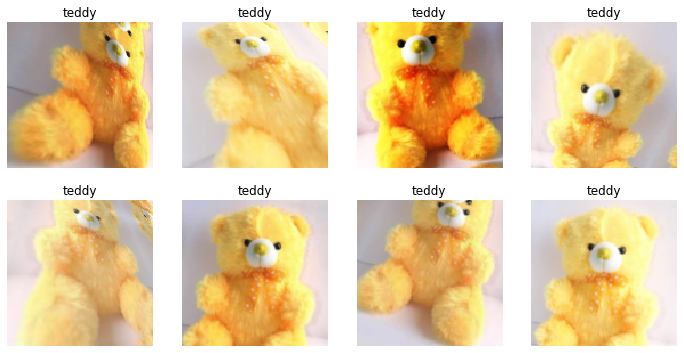
\includegraphics[width=0.6\textwidth]{imgs/data_augmentation.png}
\caption{ La librería fastai provee una forma de realizar \textit{Data Augmentation} en la GPU, acelerando considerablemente el entrenamiento. Fuente: \cite{fastbook}.  }
\label{fig:data-augmentation-image-fastai}
\end{figure}

También existen métodos estadísticos generales de \textit{data augmentation}. Por ejemplo el agregado de ruido en función a la distribución de los datos, que son aplicables a diversos tipos de datos (imágenes, sonido, vector de características, etc). Además existen métodos más avanzados como las Redes Generativas Adversiales capaces de aprender la distribución intrínseca de los datos, y a partir de ello generar datos sintéticos.\\

\begin{figure}[h!]
\centering
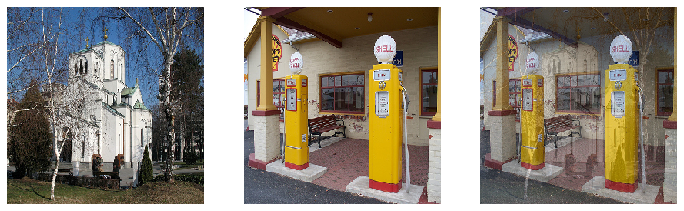
\includegraphics[width=0.6\textwidth]{imgs/mixup_result.png}
\caption{ Un ejemplo de la técnica \textit{Mixup} que combina ponderadamente dos imágenes (estación de gasolina y templo). Fuente: \cite{fastbook}  }
\label{fig:data-augmentation-mixup}
\end{figure}

Un método simple que arroja muy buenos resultados en problemas de clasificación, utilizado en Aprendizaje Profundo, es la técnica de \textbf{Mixup}  \cite{mixup} que consiste en generar nuevos ejemplos a partir de hacer un promedio ponderado entre dos datos (ver ejemplo figura \ref{fig:data-augmentation-mixup}). El mismo promedio, con igual ponderación, se aplica a las etiquetas para generar una nueva etiqueta sintética respectiva. Ver formulación matemática en la figura \ref{fig:data-augmentation-mixup-formula}.

\begin{figure}[h!]
\centering
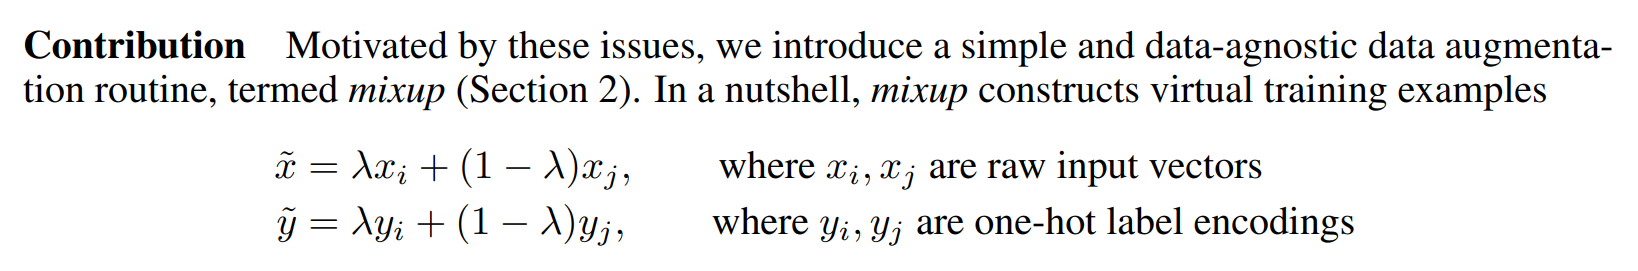
\includegraphics[width=1\textwidth]{imgs/mixup_formula.png}
\caption{ La formulación matemática de \textit{Mixup} según \cite{mixup}.  }
\label{fig:data-augmentation-mixup-formula}
\end{figure}

\subsubsection{\textit{Batch normalization}} \label{subsubection:batch-normalization}

Un problema que causa entrenamientos infecientes es el denominado \textit{\textbf{``internal covariance shift''}} explicado en \cite{batch-normalization}: la entrada de cada capa cambia conforme se entrenan las capas anteriores, por lo cuál le costará aprender los pesos definitivos hasta que las capas anteriores hayan \textit{convergido suficientemente}. Podemos pensar intuitivamente que desde la perspectiva de cada capa es como si \textit{``le cambiaran el conjunto de datos''} todo el tiempo.

Una ingeniosa manera de ver esto es en las gráficas propuestas en el capítulo 13 de \cite{fastbook} donde se grafica mediante mapa de color los histogramas de los valores de activación en función a iteraciones de entrenamiento. Como se puede ver en la figura \ref{fig:histogramactivation} las activaciones comienzan casi todas en cero. Luego, cíclcicamente, incrementan su valor exponencialmente y vuelven a cero (como si volvieran a comenzar).

\begin{figure}[H]
\begin{subfigure}{0.45\textwidth}
\centering  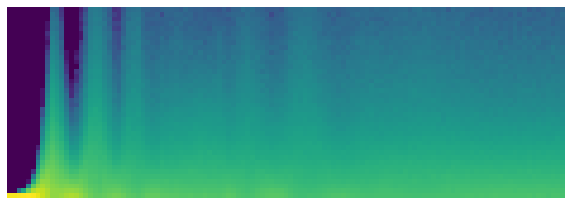
\includegraphics[width=0.8\textwidth]{imgs/histogram_activation1.png}
\end{subfigure}

\begin{subfigure}{0.45\textwidth}
\centering 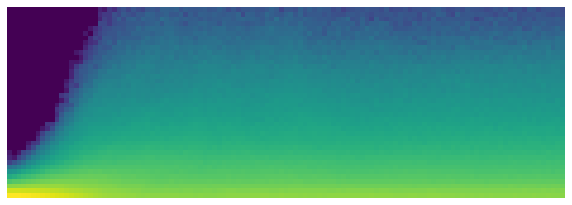
\includegraphics[width=0.8\textwidth]{imgs/histogram_activation2.png}
\end{subfigure}

\caption{ Se grafica para cada valor de activación (eje y) su cantidad en un hisotrama (color, el cero corresponde a colores más oscuros), conforme avanzan las iteraciones (eje x). En la primer figura se muestra un entrenamiento sin regularización. Se puede observar como las activaciones aumentan muy velozmente y vuelven a cero cíclicamente. En la segunda figura, luego de aplicar \textit{batch normalization}, este comportamiento desaparece: el aumento de los valores de las activaciones es más lento y consistente.  Fuente: capítulo 13 de \cite{fastbook}.  }

\label{fig:histogramactivation}
\end{figure}

Como solución a eso \cite{batch-normalization} propone normalizar cada capa de activaciones para que tengan media 0 y varianza 1. De modo de reducir ese cambio en la varianza de capas internas (\textit{internal covariate shfit}). Sobre la salida de activaciones $h_i$ de cada mini-batch se calcula su media $\mu$ y varianza $\sigma^2$ y se normaliza según:

\begin{equation*}
    BN(h_i) = \frac{h_i - \mu }{\sigma}
\end{equation*}

Para no limitar la capacidad del modelo a producir activaciones más grandes, se introducen dos parámetros \textit{entrenables} $\gamma$ y $\beta$. Serán optimizados por el método de entrenamiento como cualquier otro peso. Así se permite \textit{aprender} la media y varianza de la salida:

\begin{equation*}
    out_i = \gamma~BN(h_i)  + \beta
\end{equation*}

El método de Batch normalization hace más estable el entrenamiento, permitiendo incrementar el \textit{learning rate} y entrenar más rápidamente (menos iteraciones). También parece generar modelos que generalizan mejor, probablemente por la introducción de estocasticidad (que el modelo tiene que superar volviéndose más robusto) por la variabilidad de $\mu$ y $\sigma^2$ de las activaciones entre diferentes \textit{mini-batches}.

En el figura \ref{fig:histogramactivation} es evidente el cambio en la estabilidad de las activaciones conforme avanzan las iteraciones luego de aplciar \textit{batch normalization}.

\subsubsection{\textit{Weigth decay}} \label{subsubsection:wd}

Técnica introducida por \cite{weight-decay} que consiste en añadir un término al error que penalice la suma de los cuadrados de los pesos:
\begin{equation*}
    J_{Weight~Decay}(W) = J(W) + \lambda \sum W_i^2
\end{equation*}

$\lambda$ es un hiperparámetro que controlará la cantidad de penalización aplicada. Valores más altos entorpecerán un poco más nuestro entrenamiento pero harán que el modelo resultante generalice mejor.

Esto incentiva elegir pesos pequeños. La razón detrás de ello es que pesos grandes generan mínimos afilados en la función de costo que, como se mostró, generalizan mal. Un argumento intuitivo se expone en la figura \ref{fig:weight-decay}.

\begin{figure}[h!]
\centering
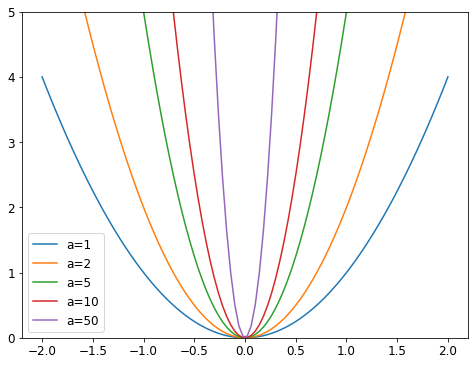
\includegraphics[width=0.6\textwidth]{imgs/weight_decay.png}
\caption{ Al aumentar $w$ en la fórmula $w x^2$ la parábola se vuelve más ``afilada''. Fuente: capítulo 8 \cite{fastbook}. }
\label{fig:weight-decay}
\end{figure}

Es fácil ver que el término de penalización en la función de costo agregará un término de $2 \alpha W_i$ sobre los gradientes de cada peso. En la práctica no se añade explícitamente el término a la función de costo sino que se modifica el cálculo de la actualización de los pesos agregando un factor de $W_i$:
\begin{equation*}
    \Delta W_i = - \eta \nabla J(W)_i - \eta \lambda w_i
\end{equation*}
O también se lo puede agregar en el cálculo del gradiente:
\begin{equation*}
    \nabla \hat{J}(W)_i = \nabla J(W)_i + \lambda w_i
\end{equation*}
Ambas son equivalentes para el método de descenso por gradiente estocástico pero en el trabajo desarrollado por \cite{decouple-weight-decay} se recomienda la segunda cuando se aplica en combinación con las técnicas momentum o Adam, debido a que es más fiel a la formulación original, y también muestra mejores resultados prácticos.

\subsubsection{\textit{Dropout}}

Es una técnica de regularización introducida en \cite{dropout}  que consiste en desactivar aleatoriamente ciertas neuronas (llevando su respectiva activación a $0$) durante el entrenamiento. Ver figura \ref{fig:dropout}.

\begin{figure}[h!]
\centering
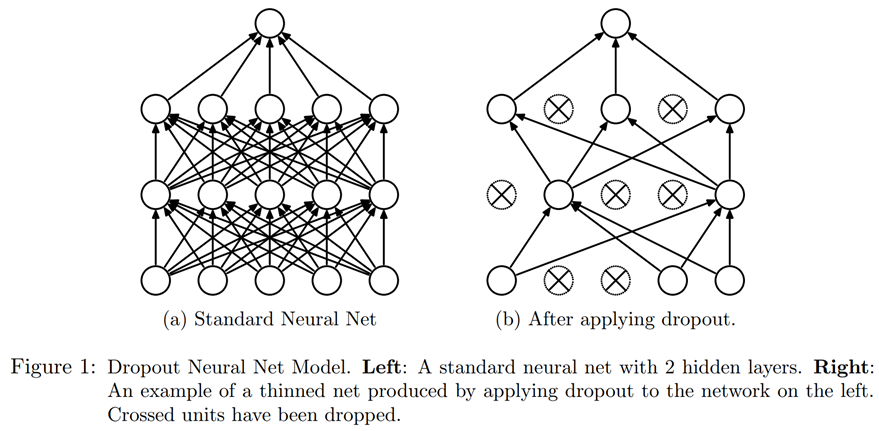
\includegraphics[width=0.9\textwidth]{imgs/dropout.png}
\caption{ Imagen esquemática extraída de \textit{``Dropout: A Simple Way to Prevent Neural Networks from Overfitting''} \cite{dropout}. }
\label{fig:dropout}
\end{figure}


La técnica funciona asombrosamente bien y ha generado un salto en el estado del arte del aprendizaje profundo. La intuición detrás de ella es que:
\begin{itemize}
    \item Mejora la cooperación entre neuronas impidiendo que intrincadamente neuronas de diferentes capas aprendan funciones de ``memorización'' del conjunto de entrenamiento. Incentivando que aprendan a extraer verdaderas características útiles y robustas.
    \item Introducen ruido en las activaciones, haciendo que se aprendan características más robustas en cada capa.
\end{itemize}

El \textit{dropout} se aplica sobre determinadas capas e incluso se ha mostrado su utilidad aplicándolo sobre la entrada para introducir ruido. Ésto puede pensarse como un caso de \textit{data augmentation}.

Notar que el apagado de las neuronas de una capa con probabilidad $p$  durante el entrenamiento requiere que se escale las salidas restantes en $\frac{1}{1-p}$. De lo contrario la capa posterior recibiría en promedio $p$ activaciones en 0 más durante el entrenamiento que durante fase de validación o durante la inferencia, lo que generaría diferentes valores promedios de activación en el entrenamiento respecto de validación, y arruinaría totalmente la generalización.

\subsection{Configurando el \textit{Learning Rate}}

Como se explicó en el apartado \ref{subsubsection:learning-rate}, el \textit{learning rate} es uno de los parámetros más importantes en el Aprendizaje Profundo: de ser muy pequeño el modelo puede tardar demasiado en entrenar, y de ser muy grande el entrenamiento puede diverger.

Optimizadores tales como Adam (explicado en el apartado \ref{subsubection:adams}) permiten escalarlo adecuadamente según el valor del gradiente. Pero notar que aún utilizando Adam, es necesario la elección del \textit{learning rate} inicial. Siendo el escalamiento aplicado por Adam independiente del valor inicial elegido.

Otras optimizaciones como \textit{Batch Normalization} (apartado \ref{subsubection:batch-normalization}) y \textit{Weight Decay} (apartado \ref{subsubsection:wd}), mitigan los riesgos de divergencia existentes derivados de utilizar valores de \textit{learning rate} elevados. No obstante, no resuelven el problema de escoger un valor inicial.

\subsubsection{Seteando el \textit{Learning Rate} inicial}

Cansado de que el modo de hallar el \textit{learning rate} óptimo sea cuestión de prueba y error, generalmente utilizando métodos como \textit{Grid Search} que requieren re-entrenar el modelo varias veces (consumiendo demasiado tiempo), Leslie N. Smith\footnote{\textbf{Nota:} Leslie N. Smith se doctoró en Química Cuántica en la Universidad de Illinosis y es investigador del \textit{Naval Research Laboratory} de los Estados Unidos. Se introdujo al Aprendizaje Profundo en 2013 y sus estudios han contribuído en hallar técnicas para entrenar más rápido y con menos datos. Este es un paso fundamental a la hora de democratizar la Inteligencia Artificial y volverla más accesible a más personas (y no solo un puñado de grandes compañías). Veáse esta entrevista que hizo para Jeremy Howard: \url{youtube.com/watch?v=dxpyg3mP_rU}}, en \cite{lr-finder}, describe un ingenioso método para encontrar el \textit{learning rate} inicial que denominó \textit{Range Test}. \footnote{También es conocido bajo el nombre de \textit{Learning Rate Finder} por la biblioteca de Aprendizaje Profundo FastAI, la cual popularizó el método usándolo en su implementación. }
El mismo consiste en probar \textit{learnings rates} incrementales (desde un valor pequeño como $10^4$) e ir aumentándolo conforme avanzan las iteraciones (para siguientes \textit{mini-batches}) hasta que el valor de la función de costo empieze a aumentar demasiado indicando divergencia (ver figura \ref{fig:lrfinder}). Luego, se corrobora empíricamente que un buen \textit{learning rate} inicial resulta de elegir un orden de magnitud por debajo del mínimo o un valor luego del cual se presente una caída abrupta del costo. Intuitivamente, para este valor la función de costo sigue decreciendo.

\begin{figure}[h!]
\centering
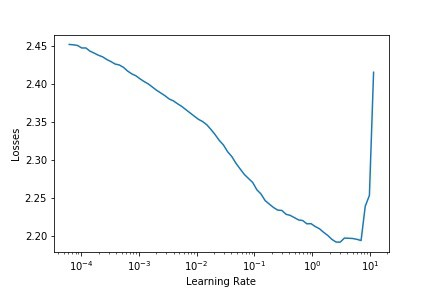
\includegraphics[width=0.6\textwidth]{imgs/lrfinder.jpeg}
\caption{ La librería FastAI provee un método denominado \textit{Learning Rate Finder} que ejecuta el test descripto en \cite{lr-finder} y muestra la gráfica de la función de costo a medida que se aumenta el \textit{learning rate}. En este caso particular una elección de \textit{learning rate} posible oscila entre $10^{-1}$ y $0.5$ (un orden de magnitud menor que el mínimo). Fuente: \href{https://github.com/fastai/fastai}{fastai}  }
\label{fig:lrfinder}
\end{figure}

\subsubsection{\textit{Cycle Learning Rates}}

Una técnica utilizada es hacer descender el \textit{learning rate} a medida que avanza el número de iteraciones, intuitivamente, para que al acercarse al minimo no se ``saltase'' por ensima de él.

En \cite{lr-finder} se sugiere hacer oscilar el valor del \textit{learning rate}, en cada época, entre dos umbrales (ver figura \ref{fig:clr}). La experimentación muestra que así se logran convergencias más rápidas.

\begin{figure}[h!]
\centering
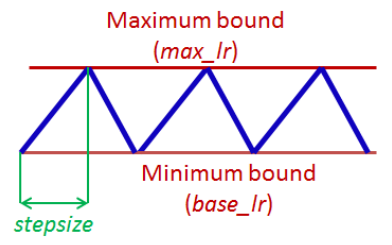
\includegraphics[width=0.4\textwidth]{imgs/clr.png}
\caption{ Imagen esquemática extraída de \cite{lr-finder}. Se halla empíricamente que incrementando y decrementando cíclicamente el \textit{learning rate} se obtienen entrenamientos más veloces y modelos que generalizan mejor.   }
\label{fig:clr}
\end{figure}

Una de las razones intuitivas es que permite superar puntos de ensilladura (ver ejemplo figura \ref{fig:saddle}). Los puntos de ensilladura son un obstáculo para el método de descenso por gradiente, ya que son zonas planas, difíciles de superar, y por ende, donde el entrenamiento se ve realentizado. Además, según reporta \cite{ensilladura}, son mucho más frecuentes que los mínimos locales en las topologías de funciones de costo.

\begin{figure}[h!]
\centering
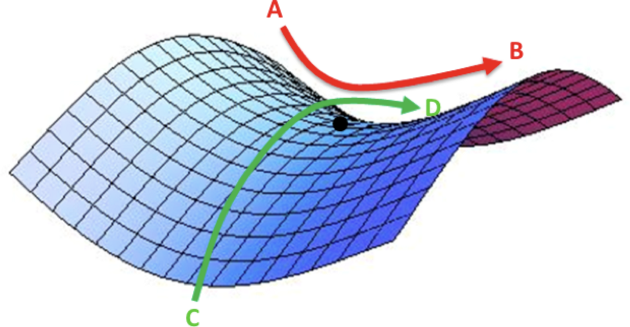
\includegraphics[width=0.4\textwidth]{imgs/saddle.png}
\caption{ Punto ensilladura para una entrada 2-dimensional. Créditos de la imágen \href{https://www.safaribooksonline.com/library/view/fundamentals-of-deep/9781491925607/ch04.html}{safaribooksonline} }
\label{fig:saddle}
\end{figure}

En \cite{leslie-2}, se ha reportado mejoras significativas en la velocidad de entrenamiento aplicando ésta técnica (utilizando en CIFAR-10 y CIFAR-100 y la familia de ResNets). El autor ha denominado a este fenómeno ``Super - Convergencia''. \cite{leslie-3}

\subsubsection{\textit{One Cycle Policy}}

Finalmente en \cite{leslie-final}, L. Smith sugiere un política de único cíclo por época para variar el \textit{learning rate}: comenzando con valores pequeños, aumentando al principio del ciclo y disminiyéndolo sobre el final (ver figura \ref{fig:one-cycle}.a). Además fija el tamaño del ciclo un poco menor al número de iteraciones de una época, y en las últimas iteraciones disminiye progresivamente el \textit{learning rate} hacia 0 (esta idea está inspirada en \textit{``Simulated Annealing''} \cite{sa}).


\begin{figure}[h!]
\begin{subfigure}{0.45\textwidth}
\centering 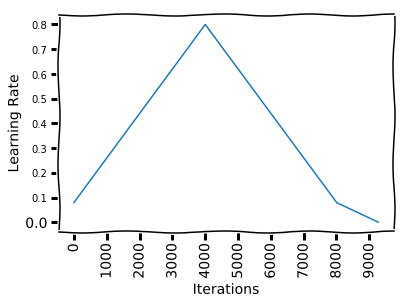
\includegraphics[width=0.45\textwidth]{imgs/onecycle_lr.png}
\end{subfigure}
\begin{subfigure}{0.45\textwidth}
\centering 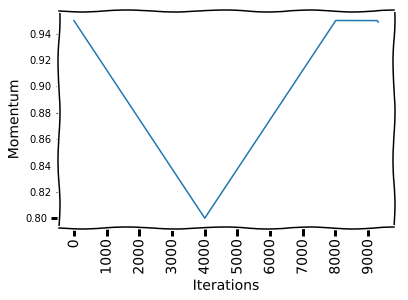
\includegraphics[width=0.45\textwidth]{imgs/onecycle_momentum.png}
\end{subfigure}
\caption{ En la imágen podemos observar cómo varía el \textit{learning rate} (izquierda) y \textit{momentum} (derecha) según la Política de Único Cíclo descripta en \cite{leslie-final}. Créditos de la imágen: \href{https://towardsdatascience.com/finding-good-learning-rate-and-the-one-cycle-policy-7159fe1db5d6}{\textit{``Finding Good Learning Rate and The One Cycle Policy''}}, autor Nachiket Tanksale.}
\label{fig:one-cycle}
\end{figure}

En \cite{leslie-final} se corroboran mejores resultados de variar el \textit{momentum} de manera inversa a la variación del \textit{learning rate}: comenzando por el umbral máximo, reduciéndolo y luego aumentándolo (ver figura \ref{fig:one-cycle}.b). Para finalmente utilizar el valor máximo de \textit{momentum} para la fase de \textit{annealing} del \textit{learning rate}

La intuicion detrás de ello es que en los momentos donde el \textit{learning rate} se está aumentando para superar puntos de ensilladura, uno desearía que el algoritmo de descenso por gradiente rápidamente vaya hacia nuevas direcciones, para lo cual es necesario que tenga baja inercia. 
 
Otra forma de entender por qué es razonable variar el \textit{momentum}, se desprende de observar la fórmula del mismo (presentada en el apartado \ref{subsubsection:momentum}) y notar que $1-\beta$ ($\beta$ es el \textit{momentum}) tiene un impacto similar a $\lambda$ (\textit{learning rate}) en la actualización de los pesos:

\begin{equation*}
    m_t = \beta~m_{t-1} + (1-\beta) (- \eta~\nabla J(w_t))
\end{equation*}

Por lo que es razonable que si en nuestra política variamos $\lambda$ querremos que $\beta$ variase en sentido opuesto (y que no nos ``contrarreste'' la variación).\\

En \cite{leslie-final} se reportan mejoras en la velocidad de entrenamiento de \textit{ResNet-50} para el dataset CIFAR-10 y CIFAR-100 de hasta $\times 10$. Además se obseva que los modelos generalizan mejor (presentan mejores resultados de validación). Esto es atribuído, a que entrenando con \textit{learnings rates} más altos se encuentran mínimos más suaves, ya que de encontrar uno empinado probablemente se ``salte'' fuera del mismo. Como se explicó en el apartado \ref{subsubsection:sharped-mins} los mínimos suaves generalizan mejor. Una vez que -aumentando progresivamente el \textit{learning rate} para evitar divergencia- se encuentran zonas con mínimos más suaves, la fase de disminución progresiva hace que encontremos la mejor parte de dicha zona (la de menor costo).

\subsection{Aprendiendo las representaciones} \label{subsection:representaciones}

Anteriormente al Aprendizaje Profundo los sistemas solían tener una fase de extracción de características que luego eran suministradas a un algoritmo de Aprendizaje Automático para entrenar \cite{dlpytorch}. La primer fase era dependiente del dominio: necesitaba ingeniería de características propia para cada problema (para imágenes se utilizaban filtros detectores de bordes, cantidad de agujeros, etc).

Por el contrario, en el Aprendizaje Profundo las características adecuadas son \textit{aprendidas} (calculadas automáticamente) por el modelo mismo. El cual, a medida que es entrenado, produce mejores características. Usualmente las representaciones aprendidas son mejores que las que puede escribir un experto manualmente. Ver figura \ref{fig:aprender-representaciones}.

\begin{figure}[h!]

\centering
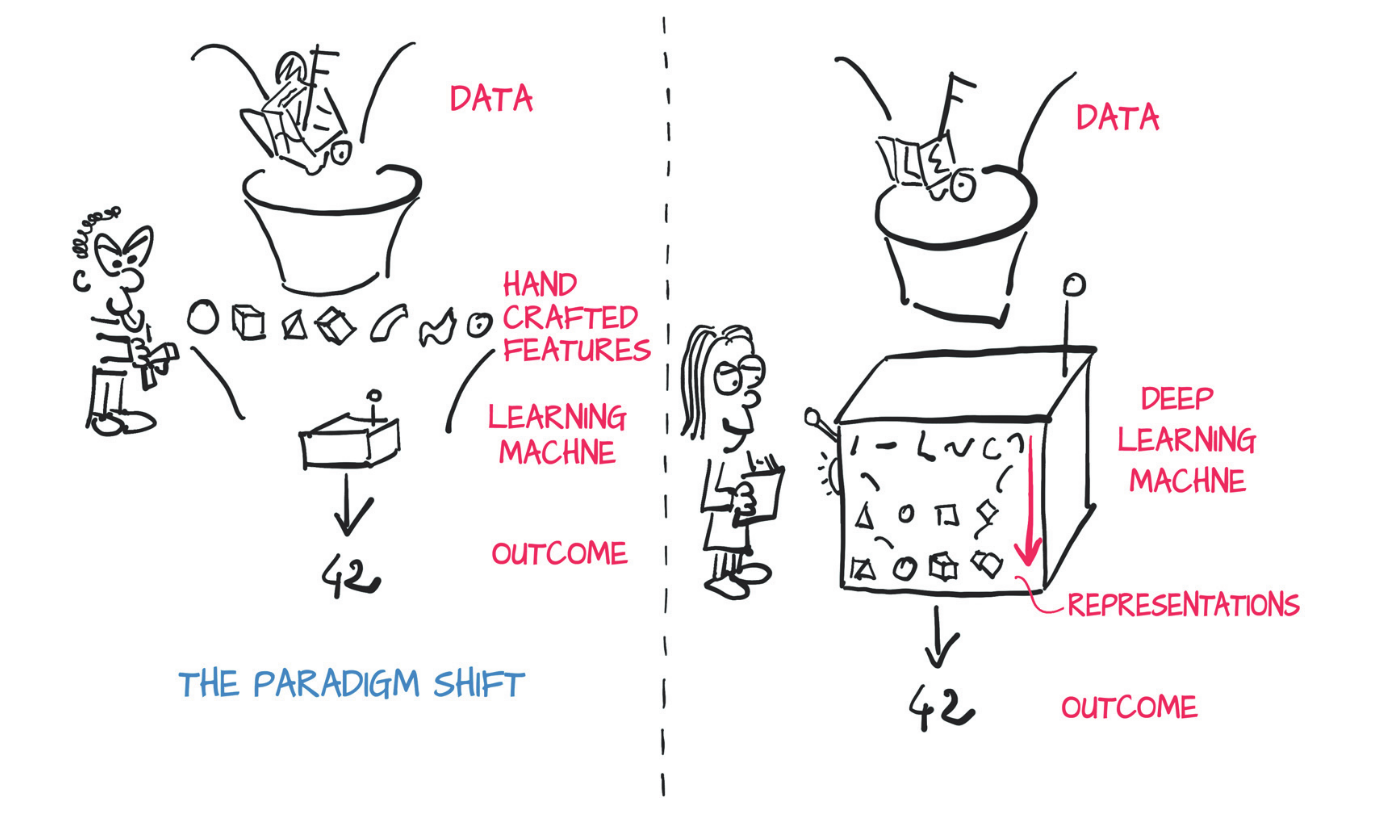
\includegraphics[width=0.65\textwidth]{imgs/learningfeatures.png}

\caption{ Imagen que esquematiza el cambio de paradigma en el Aprendizaje Automático: a la izquierda un experto del dominio se ocuapaba de programar manualmente la extracción de características. A la derecha, con el paradigma del Aprendizaje Profundo, puede focalizarse en que el modelo entrene adecuadamente para aprendarlas. Fuente: \cite{dlpytorch}}
\label{fig:aprender-representaciones}
\end{figure}

El hecho de contar con Redes Neuronales de muchas capas posibilita que las primeras aprendan representaciones más básicas, sobre las cuáles se basen las representaciones más refinadas de las capas subsiguientes. Posibilitando un paradigma que consiste en suministrarle los datos crudos al modelo (por ejemplo los píxeles de la imágen) y que no sea necesario conocimiento específico del dominio para realizar la extracción de características manualmente. Haciendo así mucho más fácilmente trasladable los métodos entre diferentes dominios de aplicación.

Éste ha sido la clave del éxito del Aprendizaje Profundo y lo que ha popularizado a las Redes Neuronales. Y fue posible gracias a que se empezó a experimentar con más de una sóla capa oculta. 

Los siguientes factores han sido clave en el desarrollo de las Redes Neuronales profundas:
\begin{itemize}
    \item El aumento en la capacidad de cómputo (sobretodo el uso de GPU).
    \item Atreverse a experimentar con más de una capa oculta (pese a las malas interpretaciones del Teorema de Aproximación Universal).
    \item El surgimiento de arquitecturas con conexiones más dispersas entre capas sucesivas: las Redes Convolucionales (que se verán en la siguiente sección), que posibilitó agregar más capas con menor costo computacional.
\end{itemize}


\subsection{Redes Neuronales Convolucionales}

Nuestro trabajo se enfocará en \textbf{Redes Neuronales Convolucionales} (\textit{CNN} del inglés \textit{Convolutional Neural Network}), arquitectura que posibilitaron modelos muy profundos de Redes Neuronales, constituyendo el primer gran éxito del Aprendizaje Profundo \cite{lenet}.\\

Se basan en dos observaciones claves, particularmente válidas para problemas de análisis de imágenes: 
\begin{itemize}
    \item Las características son \textit{locales}.  La salida de cada capa puede ser construída teniendo en cuenta solamente un área acotada de la capa anterior.
    \item Las características extraídas poseen la restricción de \textit{invariancia espacial} (\cite{lecun-invariance-shift}): cuestiones tales como detección  de bordes o texturas tienen sentido re-aplicarlas en toda la imágen. Luego, los pesos que se aplican a una zona de la imágen puede ser compartidos en otras zonas.
\end{itemize}
Estas restricciones permiten disminuir la conectividad y compartir pesos, reduciendo el número de parámetros y de computaciones realizadas en cada capa. Así, se vuelve manejable computacionalmente trabajar con muchas capas. 

Además se reduce la complejidad del modelo, reduciendo el espacio de hipótesis bajo asumpciones razonables, lo que logra una mejor generalización \cite{hipotesis1} \cite{hipotesis2}.

Así, en redes convolucionales\footnote{En el trabajo nos referiremos siempre a redes convolucionales 2-dimensionales, que son las que aplican al análisis de imágenes. Los conceptos explicados son extrapolables a entradas de más o menos dimensiones (por ejemplo existen aplicaciones de 4D CNN para videos o 1D CNN para series temporales).}, las activaciones serán matrices de dimensiones $(W,H,C)$: el ancho, la altura y la cantidad de canales respectivamente. Como capa de entrada se suministrará los pixeles de la imagen (la cantidad de canales en esta capa serán los canales de color RGB). No trabajamos con un simple vector de características, ya que nos sirve guardar el concepto de localidad (entre pixeles y las características cercanos entre sí) en la imágen original.

\subsubsection{Convoluciones}

La \textbf{convolución} es el tipo de conexión restringida entre activaciones sucesivas. Consiste simplemente en una combinación lineal de las características en una sección rectangular $(w,h)$ de la capa anterior (también se suma un parámetro de \textit{bias} $b$). Ver figuras \ref{fig:cnnkernel} y \ref{fig:cnnconv}.

\begin{figure}[h!]
\centering
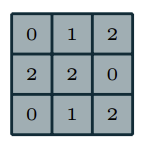
\includegraphics[width=0.1\textwidth]{imgs/cnnkernel.png}

\caption{ Ejemplo de filtro convolucional $(3,3)$. Fuente: \cite{cnn-arithmetic}}
\label{fig:cnnkernel}
\end{figure}

\begin{figure}[h!]

\centering
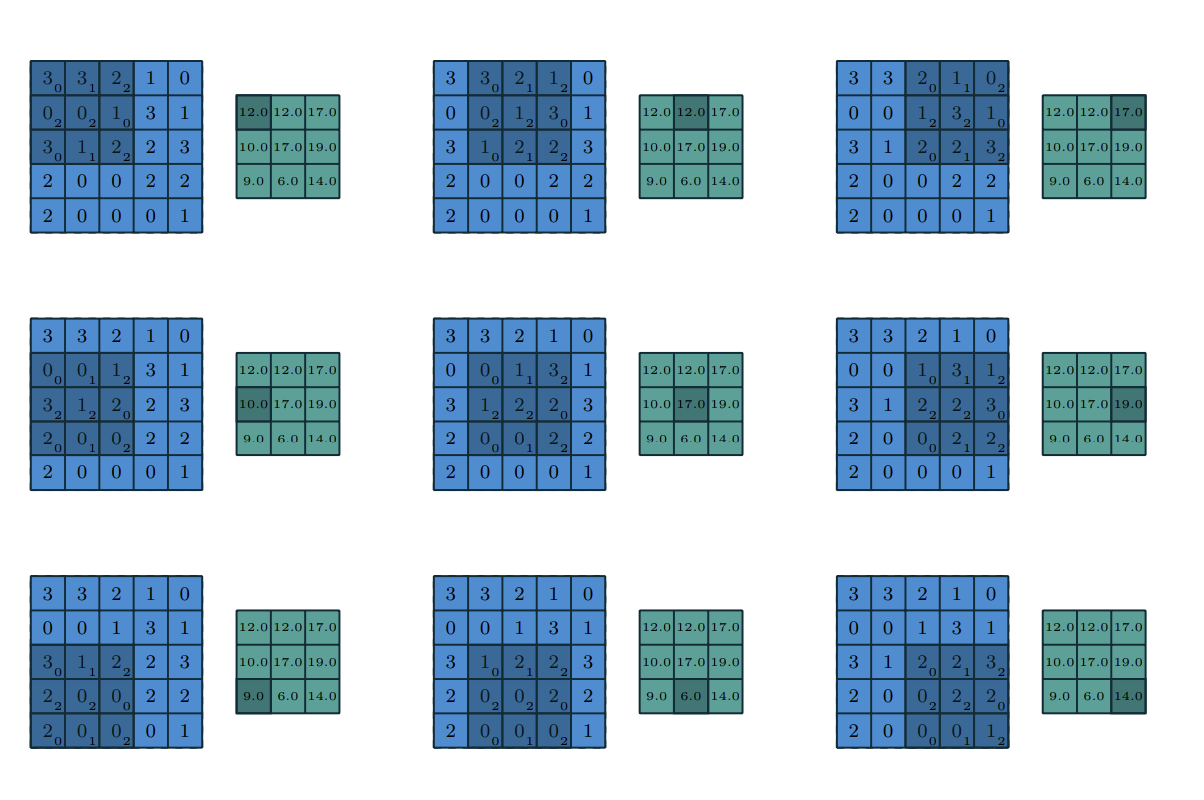
\includegraphics[width=1\textwidth]{imgs/cnnconv.png}

\caption{ El filtro de la imágen \ref{fig:cnnkernel} es aplicado a una matriz de entrada $(5,5)$ (color azul), produciendo una salida de $(3,3)$ (color aguamarina). Se han oscurecido respectivamente la zona rectangular de la matriz de entrada que interviene en la operación en cada paso, y la posición de la matriz de salida que constituye el resultado. Por razones de simplicidad hemos obviado el \textit{bias} $b$. Fuente: \cite{cnn-arithmetic}. }
\label{fig:cnnconv}
\end{figure}
Los valores de ponderación que determinan cómo se combinarán linealmente las entradas para formar las salidas son compartidos por cada salida con diferente $(W,H)$ (según \cite{lecun-invariance-shift}). La matriz $(w,h)$ con dichos valores se denomina \textit{\textbf{kernel}}. 

De tener múltiples canales de entrada ($C>1$), tendremos un filtro convolucional o \textit{kernel} para cada uno. A su vez, cada canal de  salida tiene un conjunto de filtros y \textit{bias} independiente. 

Las convoluciones ya se aplicaban en el procesamiento clásico de imágenes y eran llamadas también \textit{\textbf{filtros}}. Se usaban valores de \textit{kernels} que se sabían útiles para la extracción de ciertas características (como detección de bordes horizontales, diagonales o verticales). 

En el caso de las CNN, los \textit{filtros} serán entrenados, pretendiendo que se aprendan los valores que le resulten útiles. Además, la aplicación sucesiva de capas convolucionales apunta a que la componibilidad de los filtros sucesivos genere que la complejidad semántica de las características que se extraiga vaya en aumento con la profundidad.

\subsubsection{Aritmética de las convoluciones}

Para cada canal de la capa resultado se suman convoluciones distintas (con parámetros de \textit{kernel} distintos) de cada uno de los canales de la capa de entrada. 

Si tenemos una capa de entrada de tamaño $(W,H,c_{in})$ y le aplicamos un filtro de dimensión $(c_{out},c_{in},w,h)$ ($c_{in}$ canales de entrada, $c_{out}$ canales de salida y tamaño de kernel $w \times h$), se obtendrá una capa de salida de dimensión $(W-w+1, H-h+1, c_{out})$\footnote{Esto es considerando el caso de cero de \textit{padding} y uno de \textit{stride}. Conceptos que se explican en la subsección siguiente.}.  

Recordar que, además, tenemos un término de \textit{bias} por canal de salida ($c_{out}$ \textit{biases}, en este caso).

En el caso de las convoluciones, el número de parámetros de una capa sólo depende del tamaño del filtro: ($c_{out} \times c_{in} \times w \times h$) y el del \textit{bias}: $c_{out}$. A su vez, el número de computaciones sólo depende del producto entre el tamaño del filtro y el tamaño de la entrada. En el caso \textit{fully-connected}, tanto la cantidad de parámetros como el número de computaciones era del orden del producto de los tamaños de las activaciones sucesivas (debido a la matriz $W$). 

Esta reducción en el número de parámetros y el número de computaciones de cada capa permite entrenar modelos de muchas más capas.

Recordemos la fórmula para las capas densas (o \textit{fully-connected}) vista en la subsección \ref{subsection:nn-formulacion}:

\begin{equation*}
    f^j(\bar{h}^{j-1}) = \phi^j( {W^j}^\top \bar{h}^{j-1} + b^j)
\end{equation*}

La convolución es un caso particular de multiplicación de matrices, con restricciones sobre $W$.\footnote{Este hecho no debe sorprendernos ya que la convolución es una transformación lineal. Y las transformaciones lineales pueden ser expresadas como multiplicación de matrices.}

En la imagen \ref{fig:cnnmatmul1}.a se desgloza una convolución sobre una entrada de dimensión $(3,3)$ sobre la que se aplica un \textit{kernel} de $(2,2)$ produciendo una salida de $(2,2)$. Las combinaciones lineales dan lugar a las ecuaciones que se muestran en la figura \ref{fig:cnnmatmul1}.b. 
En la figura \ref{fig:cnnmatmul2} se muestra dicha operación como multiplicación de matrices. Notar que la matriz de la transformación (respectiva a $W$ de la fórmula vista anteriormente) posee ceros en determinadas entradas y los valores de ciertas entradas son compartidos, pueden variar según el entrenamiento pero deben ser iguales (ésto es  denominado en la jerga del Aprendizaje Profundo como \textit{shrared weights} o \textit{tied weights}).

\begin{figure}[h!]
\begin{subfigure}{0.45\textwidth}
\centering 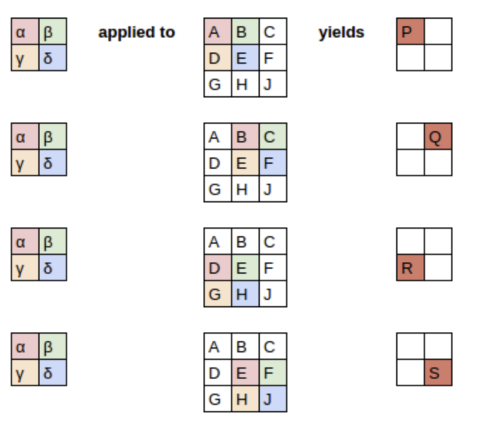
\includegraphics[width=0.5\textwidth]{imgs/cnndesgloce.png}
\end{subfigure}
\begin{subfigure}{0.45\textwidth}
\centering 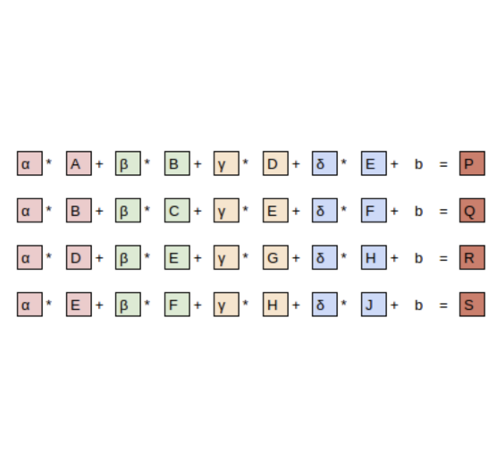
\includegraphics[width=0.5\textwidth]{imgs/cnndesgloceeqn.png}
\end{subfigure}
\caption{ A la izquierda el desgloce de la aplicación de un filtro convolucional. A la derecha las ecuaciones lineales que se desprenden de dicha convolución. El filtro está notado con las letras $\alpha$, $\beta$, $\gamma$ y $\delta$. La matriz de entrada corresponde a las letras de la $A$ a la $J$. La matriz de salida corresponde a las letras $P$, $Q$, $R$ y $S$. Fuente: \href{https://medium.com/impactai/cnns-from-different-viewpoints-fab7f52d159c}{\textit{``CNNs from different viewpoints''}}. Autor: Matthew Kleinsmith. }
\label{fig:cnnmatmul1}
\end{figure}

\begin{figure}[h!]

\centering
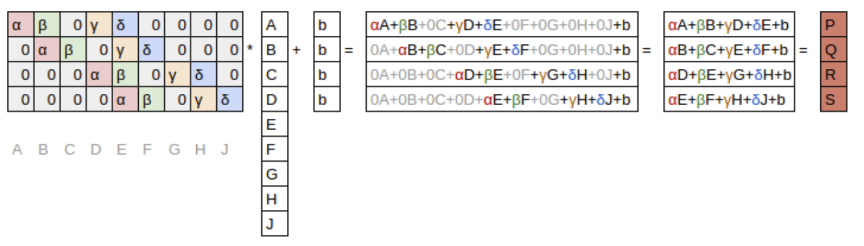
\includegraphics[width=0.85\textwidth]{imgs/cnnmatmul.png}

\caption{ Las ecuaciones de \ref{fig:cnnmatmul1}.b vistas como multiplicación de matrices. Fuente: \href{https://medium.com/impactai/cnns-from-different-viewpoints-fab7f52d159c}{\textit{``CNNs from different viewpoints''}}. Autor: Matthew Kleinsmith. }
\label{fig:cnnmatmul2}
\end{figure}

\paragraph{\textit{Padding} y \textit{Stride}}\mbox{}\\

El \textit{padding} y el \textit{stride} son hiperparámetros que configuran la convolución. Con la fórmula vista hasta ahora, el tamaño de la capa de salida está determinado por el de la entrada y el del \textit{kernel}. El propósito del \textit{padding} y el \textit{stride} es tener más flexibilidad a la hora de incidir en el tamaño de la salida.\\

El \textbf{\textit{padding}} consiste en agregar rellenos (generalmente 0) en los bordes de la capa de entrada.
Se agrega \textit{padding} para aumentar el tamaño de la salida.\\

Si pensamos a la aplicación de la convolución como un parche rectangular (el \textit{kernel}) que se va moviendo sobre la entrada (como una ventana deslizante), el \textbf{\textit{stride}} determina el tamaño del paso con el que avanza cada vez que se desplaza (ver figura \ref{fig:paddingstride}). Se agrega \textit{stride} para reducir el tamaño de la salida.

\begin{figure}[h!]

\centering
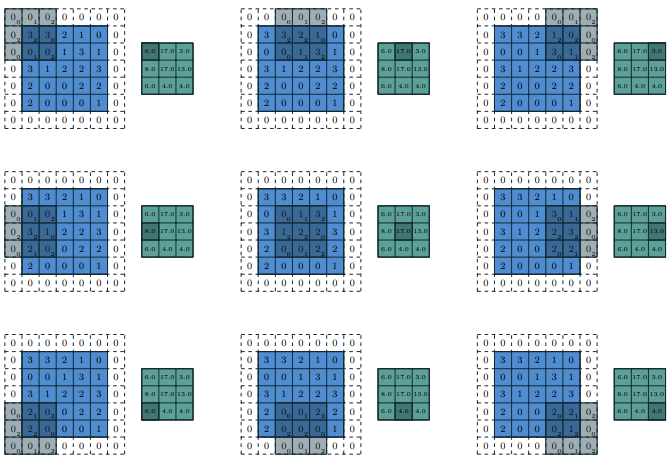
\includegraphics[width=1\textwidth]{imgs/convpadding.png}
\caption{ Ejemplo de aplicación de un \textit{kernel} convolucional de tamaño $(3,3)$ sobre una entrada de tamaño $(5,5)$ aplicando \textit{zero-padding} de $(1,1)$ y \textit{stride} de $(2,2)$. Fuente: \cite{cnn-arithmetic}}
\label{fig:paddingstride}
\end{figure}

Tanto el \textit{padding} como \textit{stride} pueden ser diferentes en el ancho o alto (aunque generalmente siempre se trabaja con cuadrados). 
En \cite{cnn-arithmetic} se muestra que si una dimensión de entrada posee tamaño $i$, y se aplica un \textit{kernel} de tamaño $k$, $p$ de \textit{padding} y $s$ de \textit{stride}, el tamaño $o$ de la salida obtenida es:

\begin{equation*}
    o = \ceil*{\frac{(i + 2p -k)}{s}} + 1
\end{equation*}

\paragraph{{\textit{Pooling}}}\mbox{}\\

Dada una entrada de tamaño $(W,H,C)$ las capas de \textit{pooling} la reducen a una capa de tamaño $(W',H',C)$ (con $W' < W$, $H' < H$), tomando el máximo (\textit{max-pooling}) o calculando el promedio (\textit{average-pooling}) de regiones rectangulares.

La reducción trabaja como una ``ventana deslizante'' que se va desplazando (al igual que el parche en la convolución) sobre la entrada. Ver figura \ref{fig:poolingexample}.

\begin{figure}[h!]
\centering
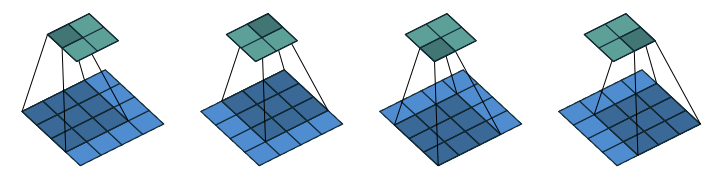
\includegraphics[width=0.85\textwidth]{imgs/convpooling.png}
\caption{ Las capas de \textit{pooling} se calculan con la misma lógica de ``ventana deslizante'' de las convoluciones. Fuente: \cite{cnn-arithmetic} }
\label{fig:poolingexample}
\end{figure}

Recomendamos \cite{cnn-arithmetic} para profundizar en el entendimiento de las convoluciones. Allí se explica y se esquematizan estos conceptos con puntillosidad.

\subsubsection{\textit{Receptive field}}

Se conoce como \textbf{área de recepción} (\textit{receptive field}) al área de la imagen original que incide sobre el cálculo de cierta activación. En \cite{fastbook} se muestra el esquema presentado en la figura \ref{fig:receptive-fields}, donde se puede ver cómo a medida que aumenta la profundidad el \textit{receptive field} es más grande. O sea que una gran porción de la imágen interviene en el cálculo de cada activación (característica) de las capas profundas. Es de esperar entonces que al aumentar la profundidad, será necesario aumentar la cantidad de filtros (canales), porque la sección de la entrada correspondiente que es representada en cada posición $(w,h)$ de la activación, es de dimensionalidad mayor. Y por ende se necesitará, probablemente, más \textit{features} para describirla.

Como se verá en el apartado \ref{subsubsection:visualizing}, las activaciones de capas más profundas corresponden a características semánticamente más complejas. Es de esperar también, que sean necesarios más filtros en las capas más profundas ya que el número de características semánticamente complejas probablemente sea mayor que el de características más simples.

\begin{figure}[h!]
\centering
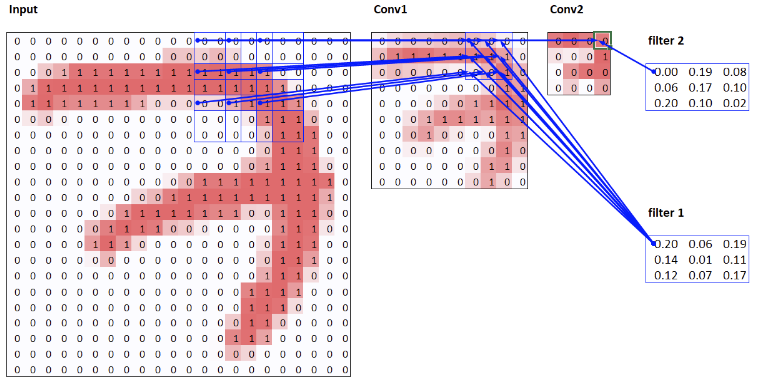
\includegraphics[width=1\textwidth]{imgs/convreceptive.png}
\caption{ En \cite{fastbook} se implementan dos capas de convoluciones en planillas de cálculo, con el fin de visualizar como el procesamiento se aplica sobre la capa de entrada (\textit{Input}) obteniendo sucesivamente las activaciones de cada convolución (\textit{Conv1} y \textit{Conv2}). \\ También se muestra la zona respectiva de la imágen para cada elemento de la salida (en azul, el \textit{receptive field}) y su relación con los filtros. \\ Fuente \cite{fastbook}. }
\label{fig:receptive-fields}
\end{figure}

A su vez en las primeras capas, el tamaño de la capa de entrada es grande, por lo que utilizar pocos filtros para ellas reducirá considerablemente el número de computaciones (que, como se dijo, es del orden del producto entre el tamaño de la capa de entrada y el tamaño del filtro).

\subsubsection{Visualizando las características aprendidas} \label{subsubsection:visualizing}

Las características aprendidas capa por capa fueron estudiadas por \cite{visualizecnn} para el modelo de cinco capas \textit{AlexNet} que ganó la competencia de \textit{ImageNet} 2012 \cite{alexnet}. Se graficó para cada capa, la intensidad de los pesos de los filtros y las partes respectivas de la imágenes (\textit{receptive fields}) para las cuáles los filtros mostraban una mayor activación (ver figura \ref{fig:visualizecnn}). 

Se observa cómo las primeras capas aprenden a reconocer características básicas (diagonales, horizontales y verticales de ciertos colores), las capas intermedias características más complejas (espirales, curvas y diferentes texturas), hasta las últimas capas que aprenden a extraer conceptos semánticos de alto nivel (flores, perros, personas, vehículos, etc).

Muchas de las características aprendidas por el modelo son parecidas a las que se solían extraer manualmente por algoritmos anteriores de análisis de imágenes. 

El trabajo nos muestra no solamente una forma de ``visualizar qué aprenden los filtros'' en las \textit{CNN}, sino también prueba el hecho de que las representaciones aprendidas son patrones deseables, componibles y de creciente complejidad.

\begin{figure}[h!]

\centering
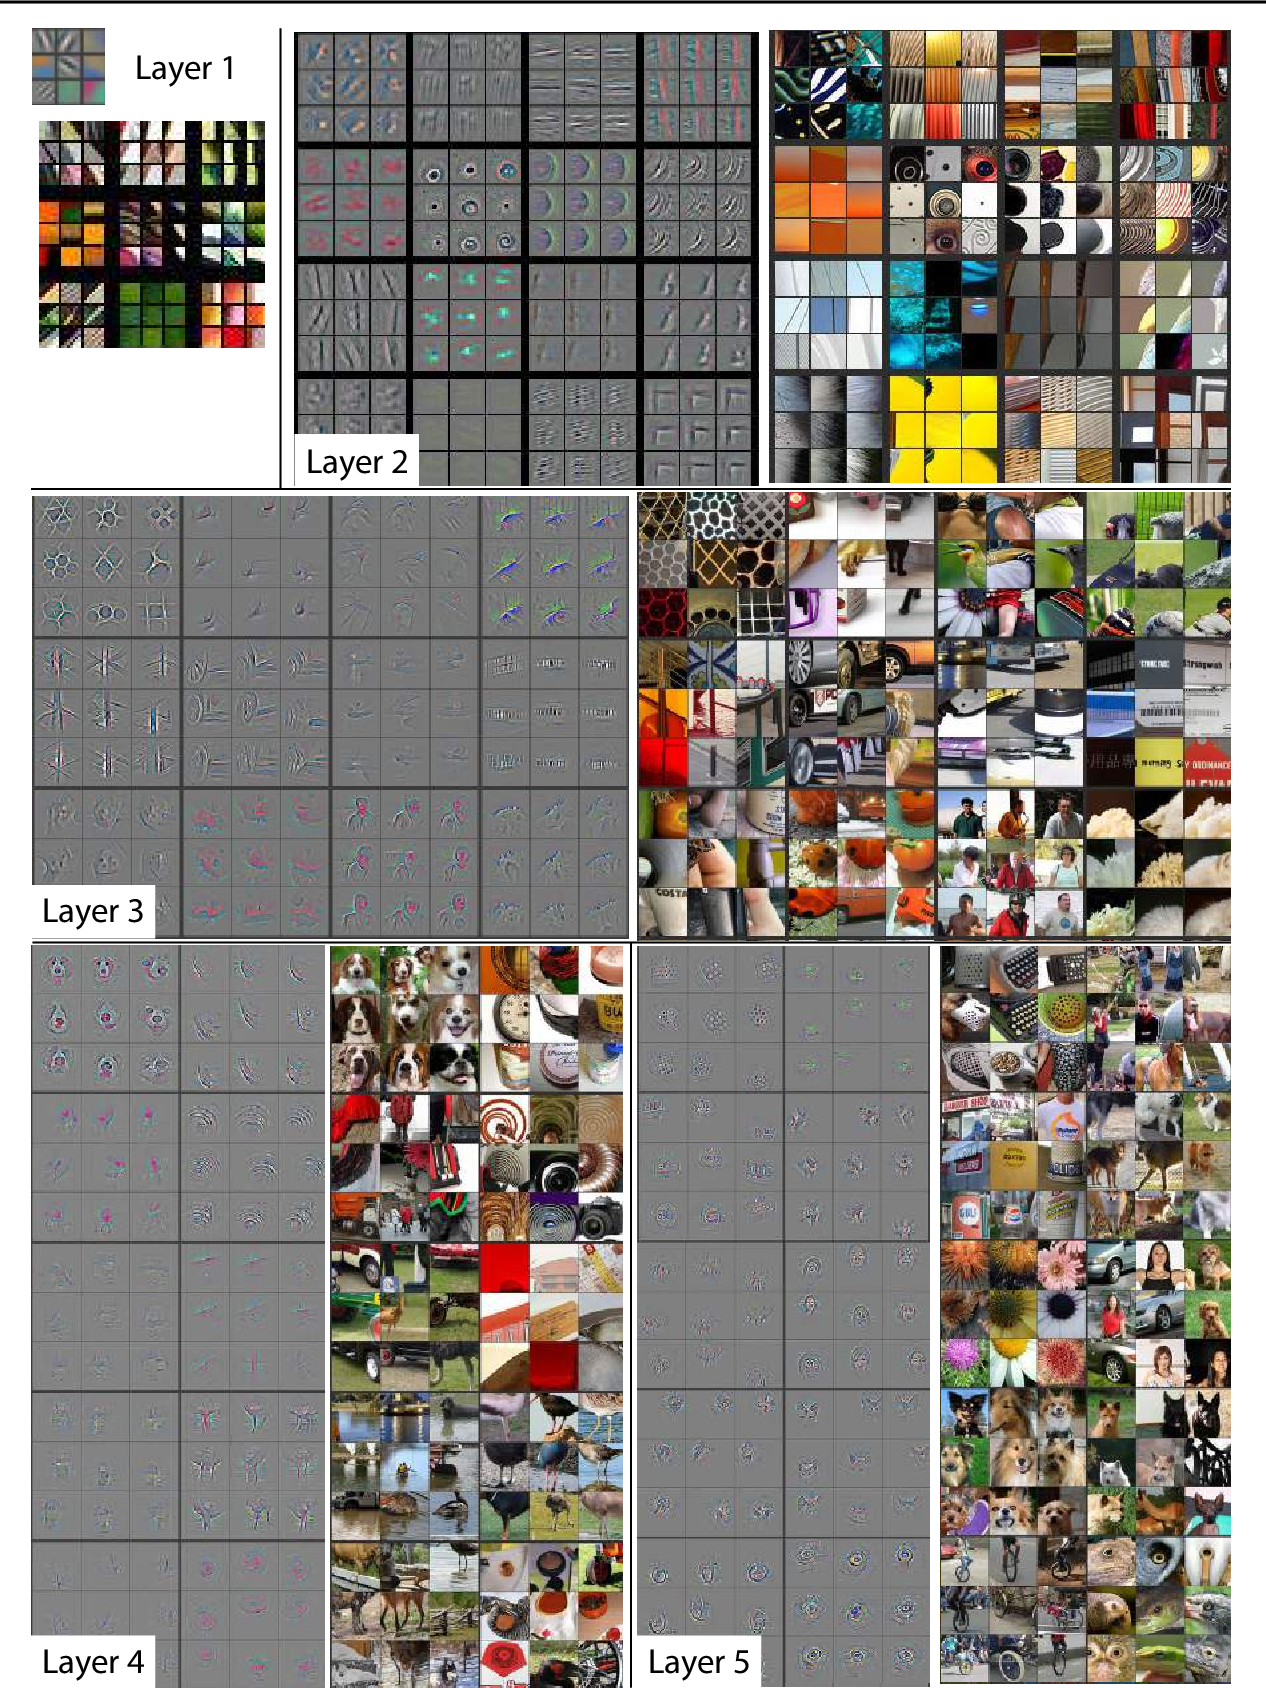
\includegraphics[width=0.98\textwidth]{imgs/visualizecnn.png}

\caption{ En gris, el valor de los filtros convolucionales. En colores, los parches de \textit{receptive field} que más activaron a los filtros respectivos. Fuente: \cite{visualizecnn}}
\label{fig:visualizecnn}
\end{figure}

\subsubsection{Redes completamente convolucionales}

Una diferencia entre las capas convolucionales y las densas (\textit{fully-connected}) está en cómo se relaciona el tamaño de la capa de entrada, el tamaño del \textit{kernel} (los parámetros) y el tamaño de la capa de salida.

Para una convolución dada, el tamaño de la entrada no depende de la misma (puede aplicarse a diferentes tamaños de entrada). Pero fijada la convolución, el tamaño de la salida será función de la entrada.

En el caso de las capas densas, dada una capa (dado $W$ y $b$), el tamaño de la entrada y la salida está completamente determinado: sólo puede aplicarse a entradas de un único tamaño, produciendo salidas de un tamaño también determinado. \\

A la hora de diseñar arquitecturas de Redes Neuronales siempre se debe pensar cómo se transforma la entrada (de cierto tamaño) en la salida (del tamaño de la predicción deseada).

Arquitecturas como \textit{VGG} (ganadora de \textit{ImageNet 2013} \cite{vgg}) apilan cierto número de convoluciones (como se dijo, con número de filtros creciente) para luego aplanar las características y aplicar una sucesión de capas densas sobre las mismas. Ésto hace que, si bien las convoluciones iniciales pueden ser aplicadas a imágenes de cualquier tamaño, la entrada de las capas densas deba ser (como se dijo) fijo. Y por ende el tamaño de la entrada original también deba ser fijo.

Una manera de evitar esta dependencia respecto del tamaño de la entrada $(W,H,C)$, consiste en apilar tantas capas de \textit{stride} (o \textit{pooling}) como sean necesarias para reducir el tamaño de la salida convolucional a $(1,1,C')$ y luego aplicar capas densas para obtener la predicción del tamaño deseado $c_{out}$. De este modo el tamaño de las capas densas sólo dependerá de $C'$, y en última instancia del número de canales de la entrada $C$, pero será independiente de $W$ y $H$.  Pero nuevamente, esto es sólo posible si conocemos el tamaño de la entrada de antemano (de lo contrario no sabríamos \textit{cuántas} capas convolucionales con \textit{stride} aplicar).\\

La solución ha sido transformar la salida de la pila de convoluciones de tamaño $(W',H',C')$ haciendo un \textit{Pooling Adaptativo},\footnote{Éstos, en vez de poseer un tamaño de ventana fijo, tienen un tamaño de salida fijo y utilizan para ello la ventana necesaria.} lo cuál escencialmente acumulará para cada canal todos los valores de las activaciones (a lo alto y ancho de la última activación), de modo de obtener una salida de tamaño $(1,1,C')$. Así, la arquitectura se mantiene totalmente desacoplada del tamaño de entrada, ya que la capa de \textit{pooling} funciona para cualquier $(W',H')$ porque es simplemente acumular los valores de cada canal usando cierta operación. 

Éstas redes se denominan \textbf{Redes Completamente Convolucionales} (\textit{FCN}, en inglés \textit{Fully Convolutional Network}). 

Luego la salida de dimensión $C'$ puede ser llevado a la predicción $c_{out}$ utilizando capas densas. Notar que $C'$ no varía si se utilizan entradas de diferente ancho o alto, ya que los canales son independientes de $W$ y $H$. Sólo depende de la cantidad de canales de entrada $C$. 

La primera parte de la arquitectura (hasta la salida de dimensión $C'$) es denominada cuerpo (\textbf{\textit{body}}). Y la segunda parte (capas densas) es llamada cabeza (\textbf{\textit{head}}). 

Estas redes pueden ser entrenadas para imágenes de cierto tamaño y usadas en imágenes de otro tamaño (notar que la cantidad de canales de la entrada debe ser el mismo).

\textbf{Nota:} la última capa del \textit{body} combina los filtros independientemente de su posición. Es importante que el dominio donde se aplique sea válido la hipótesis de \textit{invariancia traslacional}.

\subsubsection{\textit{ResNets}}

En 2015 los autores de \cite{resnet} observaron, trabajando con las ya presentadas redes \textit{VGG}, que al agregar más capas convolucionales obtenían peores valores del error y la causa no era el sobreajuste, puesto que lo mismo sucedía durante el entrenamiento (ver \ref{fig:convresnetidea}).

\begin{figure}[h!]
\centering
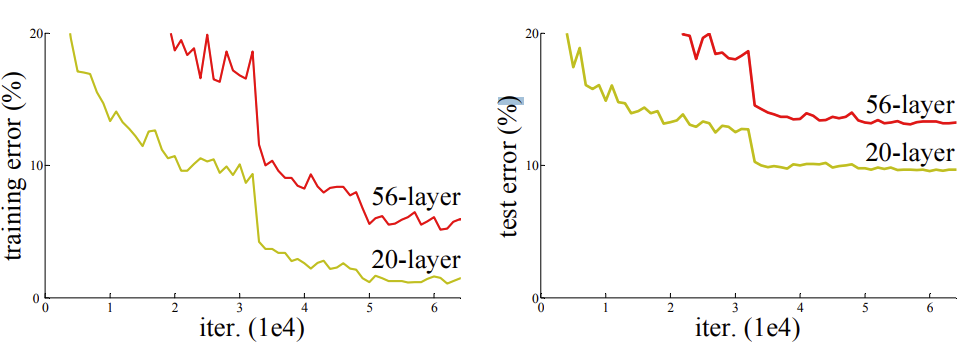
\includegraphics[width=0.85\textwidth]{imgs/convresnetidea.png}
\caption{ Observación clave que condujo al desarrollo de redes residuales. Fuente: \cite{resnet} }
\label{fig:convresnetidea}
\end{figure}

Tampoco se debía a que el cambio de arquitectura restringiera el espacio de hipótesis puesto que las capas innecesarias bien podrían aprender la identidad ($W = I$ y $b = \overline{0}$). Pero esto no sucedía: por alguna razón el algoritmo de optimización no encontraba esta solución.

Luego reemplazaron la capa de convolución:

\begin{equation*}
y = conv(x)    
\end{equation*}

Por la siguiente formulación:

\begin{equation*}
y = conv(x) + x
\end{equation*}

Además, inicializaron el parámetro $\gamma$ (de \textit{batch normalization}) en $0$. De modo que el entrenamiento podía variarlo pero inicialmente la capa era en sí la identidad. Ésta idea dio lugar al bloque que denominaron \textit{skip-connection} (ver esquema \ref{fig:convskipconn}).

\begin{figure}[h!]
\centering
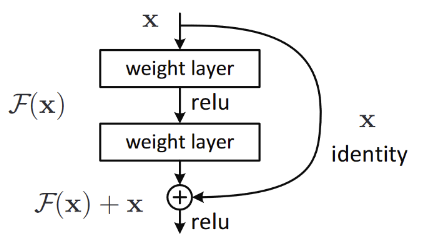
\includegraphics[width=0.5\textwidth]{imgs/convskipconn.png}
\caption{ El bloque usado en \cite{resnet} usa dos convoluciones sucesivas. La idea básica es la misma que se ha explicado: las convoluciones ahora deben aprender el \textit{residuo} de la función objetivo (menos la identidad). De modo que aprender la identidad resulta trivial. Fuente: \cite{resnet} }
\label{fig:convskipconn}
\end{figure}

En este bloque se basa la familia de \textit{Residual Neural Network} (\textit{ResNets}) ganadoras de la competencia ImageNet 2015 (\textit{error rate} $3.57 \%$), acabando con la dominancia de las \textit{VGG}. \cite{resnet}

El estudio posterior ha constatado la superioridad de estas arquitecturas. En \cite{visualizing-landscapes} se muestra que el uso de \textit{skip-connections}{ genera funciones de costo más suaves, con menos mínimos empinados (ver figura \ref{fig:visualresnetloss}) y por ende contribuyen a una mejor generalización.

\begin{figure}[h!]
\centering
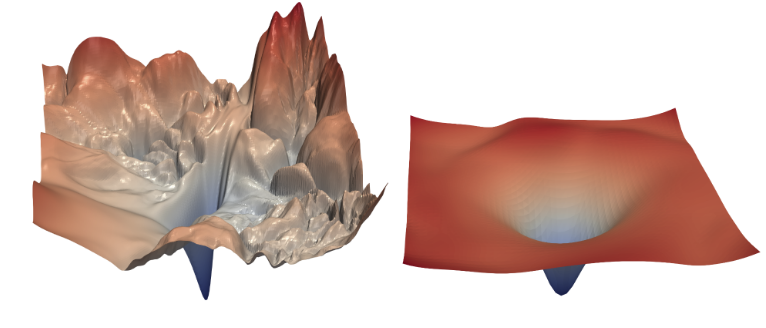
\includegraphics[width=0.85\textwidth]{imgs/convresnetsurface.png}
\caption{ Por medio de métodos de visualización lograron una representación bidimensional de la función de costo. A la derecha se ve como resulta la superficie de costo al utilizar \textit{skip-connections} Fuente: \cite{visualizing-landscapes} }
\label{fig:visualresnetloss}
\end{figure}

En \cite{cnntricks} se estudian algunos ajustes que perfeccionan la arquitectura de las \textit{ResNets}. En el trabajo se utilizan estos ajustes (incorporados a la librería FastAI). Por ejemplo se utilizan simples convoluciones en las primeras capas para mantenerlas más simples (ya que como se dijo son computacionalmente de mayor costo porque aplican a una entrada más grande). Y se reemplazan las \textit{skip-connections} por \textit{Bottlneck Layers} (ver esquema \ref{fig:bottleneck}) que son más rápidos permitiendo agregar más filtros.

\begin{figure}[h!]
\centering
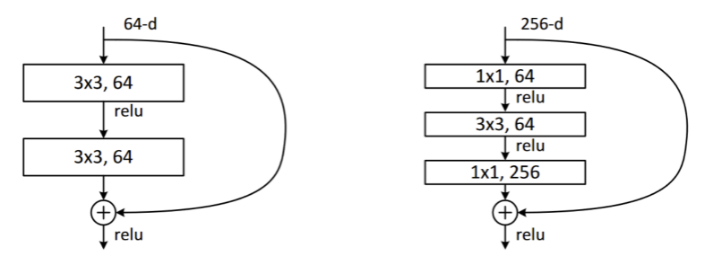
\includegraphics[width=0.8\textwidth]{imgs/convbottleneck.png}
\caption{ \cite{cnntricks} reemplaza las \textit{skip-connections} (izquierda) por \textit{Bottlneck Layers} (derecha) Fuente: \cite{cnntricks} }
\label{fig:bottleneck}
\end{figure}

\subsubsection{\textit{Fine-tuning}}

El hecho de que las características aprendidas sean patrones deseables y componibles (como se vio en el apartado \ref{subsubsection:visualizing}) da apoyo teórico a que puedan ser reutilizadas, entre problemas similares.

Se conoce como \textbf{\textit{fine-tunning}} a la técnica de transferencia del aprendizaje (\textit{transfer learning}) donde los parámetros son entrenados partiendo de la base de un modelo que ya ha sido entrenado para un conjunto de datos diferente (e incluso para un problema diferente) al que se quiere resolver.

Así, por ejemplo, si se quiere hacer un clasificador de fotografías de tipos de automóviles, se pueden obtener resultados con precisión del estado del arte aún sin contar con demasiados datos, y entrenando unas pocas épocas, si re-entrenamos un modelo ya entrando sobre el \textit{dataset ImageNet} (por ejemplo podríamos usar \textit{ResNet-50}). La técnica incluso sirve para problemas diferentes a la clasificación (por más que el problema original de \textit{ImageNet} es entrenar un clasificador), ya que lo transferible son las  de características extraídas en las capas intermedias. Por ejemplo se pueden entrenar modelos para problemas de regresión, \textit{tagging} multi-clase, etc.\\

En general cuando se aplica \textit{fine-tunning} se conserva la parte de la arquitectura que hemos denominado \textit{body} y se coloca un nuevo \textit{head}. Ésto es debido a que el \textit{head} es problema-específico, ya que depende del tamaño de la salida $c_{out}$. Además, las características codificadas por las últimas capas tendrán que ver con las cuestiones específicas del problema y lo que se quiere transferir son las representaciones que son trasladables entre los dos problemas.

La librería \textit{FastAI} posee la funcionalidad de fácilmente congelar los pesos del \textit{body}, de modo de entrenar unas épocas modificando el \textit{head} solamente (ya que al ser inicializado de cero, contendrá pesos aleatorios). Esto tiene sentido ya que no queremos que la señal de \textit{backpropagation} de un \textit{head} totalmente aleatorio arruine las representaciones útiles que intentamos transferir. Además el congelamiento de las primeras capas reduce el problema de \textit{internal covariance shift}, ya que sólo varía el \textit{head} y no las capas anteriores (su entrada). Hay quienes incluso pre-computan las activaciones de salida del \textit{body}, ya que no variarán durante esta fase, para no volverlas a calcular. Luego podemos descongelar los parámetros del \textit{body} y entrenar todo el modelo en su conjunto. \cite{fastbook}

En línea con el argumento del párrafo anterior \cite{discriminative-lr}\footnote{Jason Yosinski et al. desarrolló este método originalmente para el problema de NLP ULMFiT. Cómo muchos conceptos de Aprendizaje Profundo, es extrapolable a otras áreas.} propone asignar \textit{learning rates} diferenciados durante el proceso de \textit{fine tunning} de modo que las primeras capas (más cercanas a la entrada) no varíen tanto como las últimas. Ésto está en consonancia con el hecho de que las representaciones de las primeras capas son conceptos más simples y serán más extrapolables, en cambio las capas posteriores (incluso del \textit{body}) son más complejos y tendrán que re-adaptarse al problema específico.


\subsection{Arquitecturas de redes siamesas} \label{subsection:siamesas}

Como se discutió en el capítulo \ref{chapter:trabajos-anteriores}, muchos problemas de similitud de imágenes (por ejemplo \textit{Face Verification} o similitud de firmas) no se resuelven entrenando un clasificador con una clase por identidad, sino aprendiendo una \textit{representación} y una \textit{métrica} que permitan comparar pares de ejemplos. Las \textbf{redes siamesas} constituyen una arquitectura estándar para este tipo de problemas \cite{siamess-lecun}. La idea central es utilizar un mismo \textit{encoder} convolucional $G_W$ para mapear cada imagen $img$ a un vector de características de dimensión fija (un \textit{embedding}):
\begin{equation*}
    z = G_W(img) \in \mathbb{R}^d,
\end{equation*}
compartiendo los pesos $W$ entre ambas ramas de la red (lo que en la jerga se conoce como \textit{tied weights}). 

A partir de estos \textit{embeddings} se define una función de distancia $d(z_1, z_2)$ (por ejemplo la distancia euclídea o la distancia coseno) y se entrena el modelo para que firmas (o imágenes) de la misma clase queden “cerca” en el espacio de representación, y las de clases distintas “lejos”. Desde esta perspectiva, el clasificador binario que decide si dos firmas son de la misma autoría o no pasa a ser un umbral sobre la distancia:
\begin{equation*}
    autoresNoCoinciden(img_1, img_2) = 
    \left\{
        \begin{array}{ll}
        \text{Verdadero} & \text{si } d(G_W(img_1), G_W(img_2)) > \tau \\
        \text{Falso}     & \text{si } d(G_W(img_1), G_W(img_2)) \leq \tau
        \end{array}
    \right.
\end{equation*}
para algún umbral $\tau$ elegido según los criterios de costo–beneficio discutidos en \ref{subsubsection:costo-beneficio}. En nuestro caso particular, este esquema permite aprovechar el mismo \textit{encoder} convolucional para firmar autores nunca vistos durante el entrenamiento, algo que sería muy difícil de lograr con un clasificador “uno contra todos” por autor.

\subsubsection{Triplet loss} \label{subsubsection:triplet-loss}

Una forma efectiva de entrenar redes siamesas es mediante funciones de costo diseñadas específicamente para \textit{aprendizaje de métricas}. Entre ellas, una de las más utilizadas es la \textbf{\textit{triplet loss}}. En lugar de trabajar con pares $(img_1, img_2)$, se consideran tripletas $(a, p, n)$:
\begin{itemize}
    \item $a$ (\textit{anchor}): una firma de referencia.
    \item $p$ (\textit{positive}): una firma del mismo autor que $a$.
    \item $n$ (\textit{negative}): una firma de un autor distinto.
\end{itemize}

Sea $z_a = G_W(a)$, $z_p = G_W(p)$ y $z_n = G_W(n)$ sus \textit{embeddings}. La triplet loss impone que la distancia entre el ancla y el positivo sea menor, al menos por un margen $\alpha > 0$, que la distancia entre el ancla y el negativo:
\begin{equation*}
    L(a,p,n) = \max\big(0,\ d(z_a, z_p) - d(z_a, z_n) + \alpha \big).
\end{equation*}
Intuitivamente, el costo es cero siempre que $z_a$ esté "más cerca" de $z_p$ que de $z_n$ por al menos $\alpha$, y positivo en caso contrario. El entrenamiento busca minimizar la suma (o el promedio) de $L(a,p,n)$ sobre un conjunto de tripletas construidas a partir del \textit{dataset}. 

Cabe notar que esta formulación resulta menos restrictiva que otras funciones de costo que fuerzan a los ejemplos de una misma clase a colapsar en un único punto del espacio de representación. La triplet loss únicamente exige que los ejemplos positivos estén más cerca del ancla que los negativos, permitiendo así que las muestras de un mismo autor mantengan cierta dispersión entre sí. Esta flexibilidad es deseable en dominios como el de firmas manuscritas, donde existe variabilidad intra-clase natural y no resulta razonable pretender que todas las instancias de un autor converjan a una representación idéntica.

En la práctica es crucial la estrategia con la que se generan dichas tripletas: si se eligen tripletas “fáciles” (para las cuales la desigualdad ya se cumple ampliamente), el gradiente será casi nulo y el modelo aprenderá poco; por el contrario, seleccionar tripletas demasiado difíciles puede llevar a inestabilidades numéricas o a un entrenamiento que no converge. Existen esquemas \textit{offline} (las tripletas se pre–generan) y \textit{online} (se seleccionan dinámicamente tripletas informativas dentro de cada \textit{mini-batch}), que se describen con más detalle en el capítulo de Experimentos. En nuestro trabajo utilizamos variantes de \textit{triplet loss} precisamente para forzar que firmas de la misma autoría colapsen en regiones compactas del espacio de representación y que firmas de diferentes autores queden claramente separadas, lo que se traduce luego en mejores métricas de \textit{precision} y \textit{recall} en el problema binario definido en \ref{section:objectives}.

